\documentclass{mimosis}

\usepackage{metalogo}

%%%%%%%%%%%%%%%%%%%%%%%%%%%%%%%%%%%%%%%%%%%%%%%%%%%%%%%%%%%%%%%%%%%%%%%%
% Some of my favourite personal adjustments
%%%%%%%%%%%%%%%%%%%%%%%%%%%%%%%%%%%%%%%%%%%%%%%%%%%%%%%%%%%%%%%%%%%%%%%%
%
% These are the adjustments that I consider necessary for typesetting
% a nice thesis. However, they are *not* included in the template, as
% I do not want to force you to use them.

% This ensures that I am able to typeset bold font in table while still aligning the numbers
% correctly.
\usepackage{etoolbox}

%%%%%%%%%%%%%%%%%%%%%%%%%%%%%%%%%%%%%%%%%%%%%%%%%%%%%%%%%%%%%%%%%%%%%%%%
% Hyperlinks & bookmarks
%%%%%%%%%%%%%%%%%%%%%%%%%%%%%%%%%%%%%%%%%%%%%%%%%%%%%%%%%%%%%%%%%%%%%%%%

\usepackage[%
  colorlinks = true,
  citecolor  = RoyalBlue,
  linkcolor  = RoyalBlue,
  urlcolor   = RoyalBlue,
  unicode,
  ]{hyperref}

\usepackage{bookmark}

%%%%%%%%%%%%%%%%%%%%%%%%%%%%%%%%%%%%%%%%%%%%%%%%%%%%%%%%%%%%%%%%%%%%%%%%
% Bibliography
%%%%%%%%%%%%%%%%%%%%%%%%%%%%%%%%%%%%%%%%%%%%%%%%%%%%%%%%%%%%%%%%%%%%%%%%
%
% I like the bibliography to be extremely plain, showing only a numeric
% identifier and citing everything in simple brackets. The first names,
% if present, will be initialized. DOIs and URLs will be preserved.

\usepackage[%
  autocite     = plain,
  backend      = biber,
  doi          = true,
  url          = true,
  giveninits   = true,
  hyperref     = true,
  maxbibnames  = 99,
  maxcitenames = 99,
  sortcites    = true,
  style        = ieee, % style = numeric
  ]{biblatex}

%\input{bibliography-mimosis}
\addbibresource{references.bib}

%%%%%%%%%%%%%%%%%%%%%%%%%%%%%%%%%%%%%%%%%%%%%%%%%%%%%%%%%%%%%%%%%%%%%%%%
% Fonts
%%%%%%%%%%%%%%%%%%%%%%%%%%%%%%%%%%%%%%%%%%%%%%%%%%%%%%%%%%%%%%%%%%%%%%%%

\ifxetexorluatex
  %\setmainfont{EB Garamond}
  %\setmonofont[Scale=MatchLowercase]{Source Code Pro}
\else
  \usepackage[lf]{ebgaramond}
  \usepackage[oldstyle,scale=0.7]{sourcecodepro}
  \singlespacing
\fi

\newacronym                                            {DFP}{DFP}{Degree Final Project}
\newacronym                                            {OCR}{OCR}{Optical character recognition}
\newacronym                                            {API}{API}{Application programming interface}
\newacronym                                            {IDE}{IDE}{Integrated development environment}
\newacronym                                            {CLI}{CLI}{Command line interface}

\newglossaryentry{Hangeul}{%
  name        = {\textit{Hangeul}},
  description = {Korean language native script},
  sort        = {Hangeul},
}

\makeindex
\makeglossaries

%%%%%%%%%%%%%%%%%%%%%%%%%%%%%%%%%%%%%%%%%%%%%%%%%%%%%%%%%%%%%%%%%%%%%%%%
% Incipit
%%%%%%%%%%%%%%%%%%%%%%%%%%%%%%%%%%%%%%%%%%%%%%%%%%%%%%%%%%%%%%%%%%%%%%%%

\usepackage{lipsum}
\usepackage{kotex}
\usepackage{subcaption}
\usepackage{rotating}
\usepackage{pdfpages}
\usepackage{amssymb}

\titlehead{	
	
\includegraphics[height=25mm]{Figures/logo_ual.png}
	\hfill
	
\includegraphics[height=25mm]{Figures/logo_esi.png}
}
\subject{Grado en Ingeniería Informática}

\title{Identificación de alérgenos a partir de productos envasados para extranjeros residentes en Corea}
\subtitle{Trabajo Fin de Grado}
\author{Alonso Bravo Moyano}
\date{Curso académico 2021-2022} %September 2021 %\today

\publishers{\textbf{Directores:}\\Rafael Guirado Clavijo\\José Fernando Bienvenido Bárcena}

\begin{document}


\includepdf[]{Cover/PortadaTFG.pdf}

\frontmatter
%     \dedication{To my treasured hazel-hen\\
% in eternal love\\
% from your dormouse.}

    \maketitle
    \chapter*{Abstract}

For any patient of food allergies and intolerances, it is vital to know the composition of any food product before consumption. Although the solution is often as trivial as looking at the list of ingredients on the packaging, this task becomes much more complex if the patient is in a foreign country, where they may not know the language or be familiar with the product.

To tackle this problem, this bachelor's thesis proposes the development of a mobile application focused on the case of South Korea. This application incorporates an OCR system that allows the user to recognize the text of the packaging in Korean from the capture of a photograph of the list of ingredients. Combining a pre-built database with translation engines, the application analyzes the identified terms and will alert the user if the product includes any unwanted ingredients.

\par\vskip\baselineskip\noindent
\textbf{Keywords:} Optical character recognition (OCR), ML Kit, Flutter, allergens, Korean language

\chapter*{Resumen}

Para cualquier paciente de alergias e intolerancias alimentarias, es vital conocer la composición de cualquier producto alimenticio antes de su consumo. Aunque la solución suele resultar tan trivial como consultar la lista de ingredientes en el empaquetado, esta tarea se vuelve mucho más compleja si el paciente se encuentra en un país extranjero, donde puede no conocer el idioma ni estar familiarizado con el producto.

Para atajar este problema, en este trabajo se propone el desarrollo de una aplicación móvil enfocada al caso de Corea del Sur. Dicha aplicación incorpora un sistema OCR que permite al usuario reconocer el texto del empaquetado en coreano a partir de la captura de una fotografía de la lista de ingredientes. Combinando una base de datos preconstruida con motores de traducción, la aplicación analiza los términos identificados y alertará al usuario si el producto incluye cualquier ingrediente no deseado.

\par\vskip\baselineskip\noindent
\textbf{Palabras clave:} Reconocimiento óptico de caracteres (OCR), ML Kit, Flutter, alérgenos, idioma coreano
    \tableofcontents
    \listoffigures
    \listoftables
    

\mainmatter
    % \part[Primera parte]{%
    %     A good part\\
    %     %
    %     \vspace{1cm}
    %     %
    %     \begin{minipage}[l]{\textwidth}
    %     %
    %     \textnormal{%
    %       \normalsize
    %       %
    %       \begin{singlespace*}
    %         \onehalfspacing
    %         %
    %         \lipsum[1]
    %       \end{singlespace*}
    %     }
    %     \end{minipage}
    %   }

    \chapter{Introduction}
\label{chapter1}

One of the greatest difficulties faced by patients with allergies or other food intolerances is the proper identification of which products they can safely consume. This task becomes much more complex when the patient is in a foreign country, where the products will usually be packaged in a language different from their mother tongue. At a time when the prevalence of food allergies continues to increase \cite{tang_food_2017}, as is the number of young Spaniards emigrating abroad \cite{dominguez-mujica_international_2018}, finding an effective solution to this problem has become ever more necessary.
    
In particular, in some countries like South Korea, the language barrier for foreign residents (who only constitute a mere 3.9\% of the total population \cite{noauthor__2021-1}) represents a hurdle hard to obviate.
    
The Korean language is classified by the US Foreign Service Institute as one of the 5 most difficult languages to learn for a native English speaker, requiring up to 2200 hours of study \cite{noauthor_foreign_2021}. Furthermore, in a study based on the domain acquired after 24 weeks of study, Chiswick and Miller assigned it the maximum lexical distance from English \cite{chiswick_linguistic_2005}.

One of the main factors contributing to this difference is that Korean uses their own native alphabet, \textit{hangeul}, composed of 24 basic characters that are combined to form syllabic blocks \cite{noauthor_hangul_2021}. The Figure \ref{fig:label} depicts a real example of text in \textit{hangeul}.

\begin{figure}[h]
  \centering
  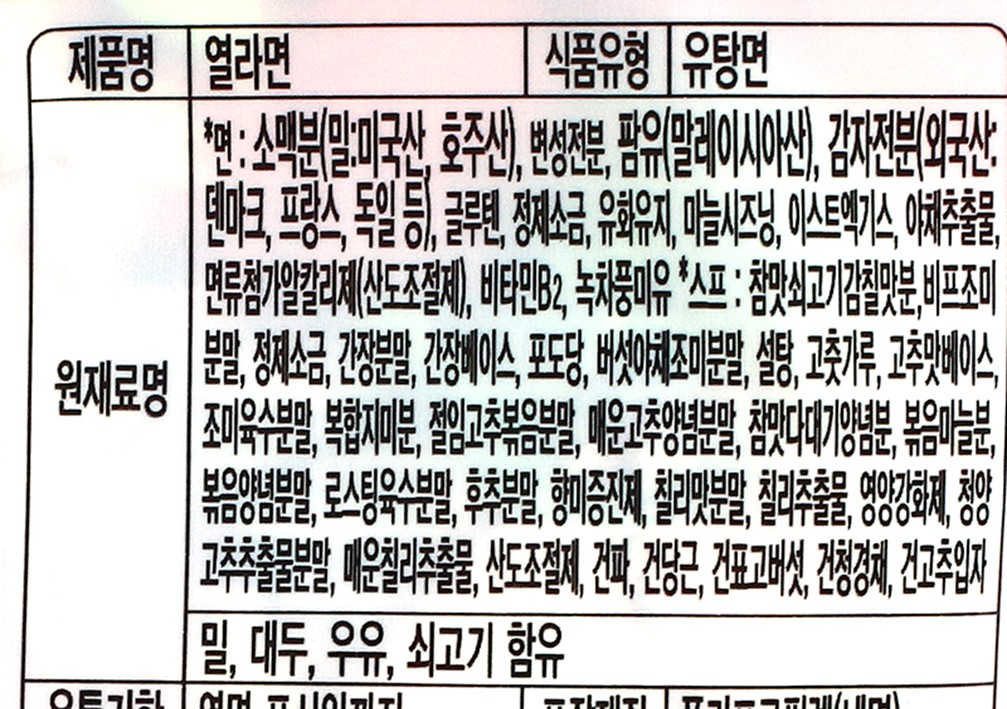
\includegraphics[width=0.5\textwidth]{Figures/label.jpg}
  \caption{%
    Label of a packaged food product in Korean
  }
  \label{fig:label}
\end{figure}

The barrier across these languages that make use of different alphabets or scripts makes basic tasks such as the input of text in a translator laborious to those who may not be familiar with the appropriate tools (Korean keyboards, OCR systems, speech-to-text, etc.). These methods, like the most commonly used shown in Figure \ref{fig:keyboard}, often require the user to have an entry-level knowledge of Korean language in general or \textit{hangeul} in particular, which may take some time to acquire for newcomers to South Korea.

\begin{figure}[h]
    \begin{subfigure}{0.5\textwidth}
        \centering
        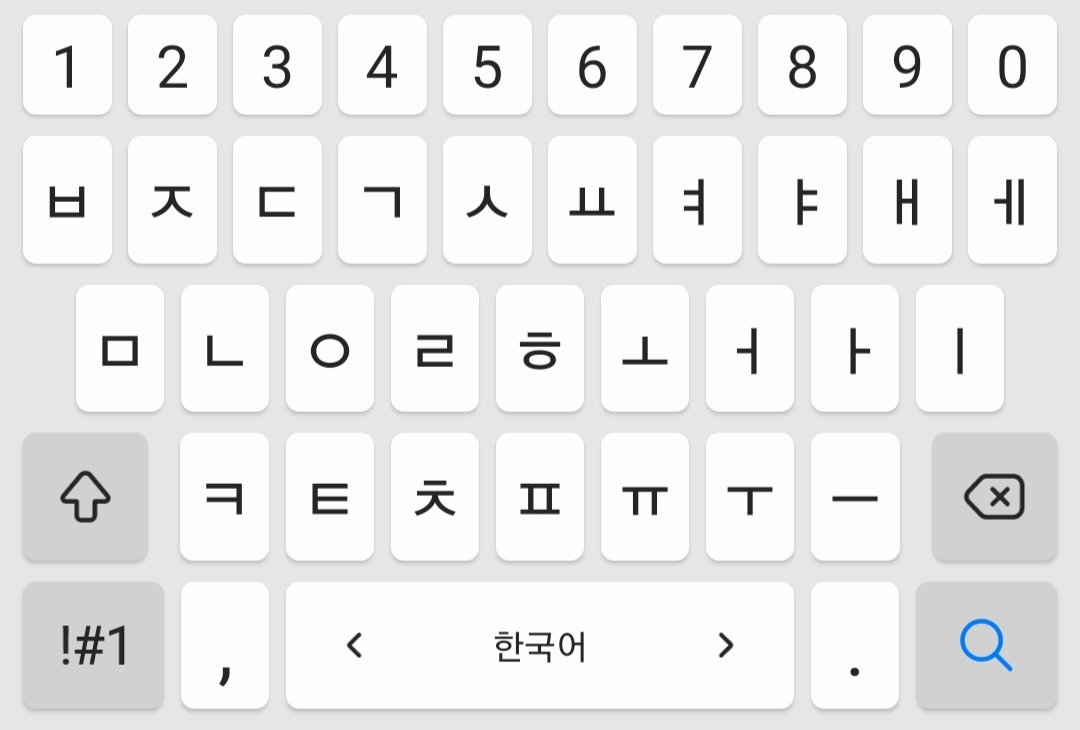
\includegraphics[width=0.9\linewidth]{Figures/2beolsik.jpg} 
        \caption{2-beolsik}
        \label{fig:2beolsik}
    \end{subfigure}
    \begin{subfigure}{0.5\textwidth}
        \centering
        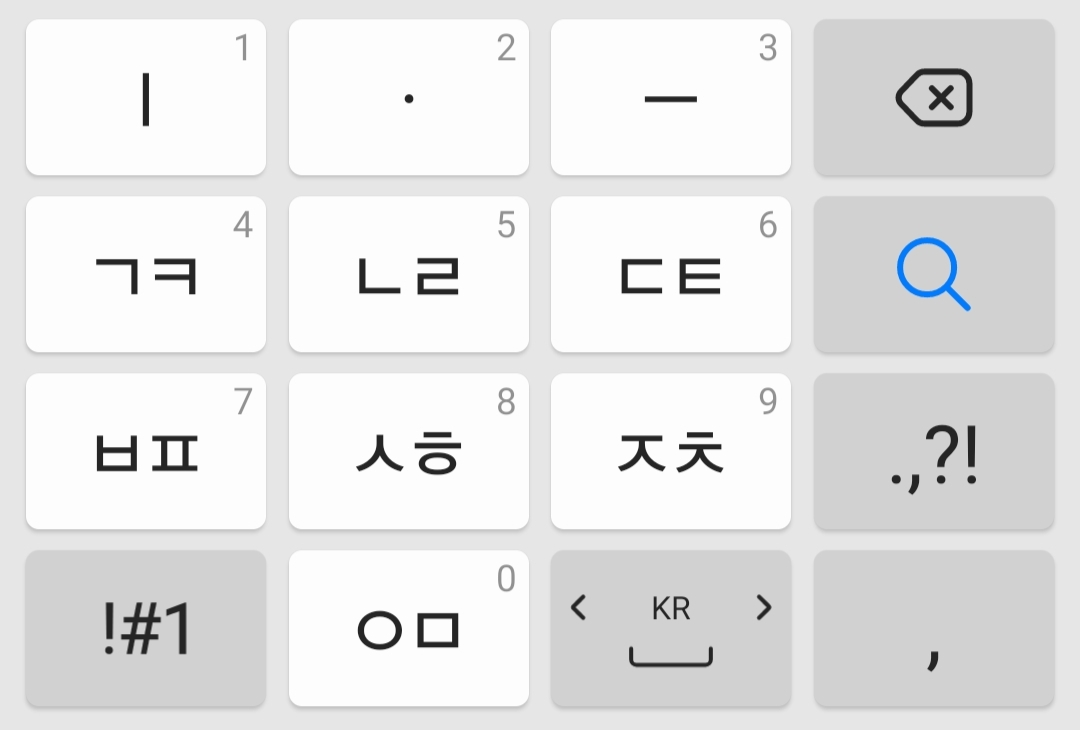
\includegraphics[width=0.9\linewidth]{Figures/chunjiin.jpg}
        \caption{Chunjiin}
        \label{fig:chunjiin}
    \end{subfigure}
    \caption{Korean keyboard layouts}
    \label{fig:keyboard}
\end{figure}

This combination of factors complicate such an elementary and vital process for an allergy patient as is understanding the labeling of a product, reading its ingredients and identifying what possible allergens it may include.

\section{Motivation}
    
To assist in this task, this Degree Final Project (DFP) will focus on producing a mobile application whose main functionality allows scanning the text in the list of ingredients for any packaged food product. Based on the substances specified by the user, the application will issue a warning if any of them are found among the recognized words.
    
This idea is mainly motivated by the experience of the author, who currently resides in South Korea, as well as by the experiences of his acquaintances with allergies and of all those to whom its use is extended: vegetarians, vegans, celiacs, lactose intolerant, consumers of halal products, \textit{kosher} products, etc. Likewise, this concept could potentially be ported to support other languages and scripts, thus increasing the target audience to every foreign person having difficulties reading labels written in language of the country where they reside.

Another relevant reason for choosing this topic for the DFP was that it represents a great opportunity to bridge the knowledge acquired through some of the courses in the degree, such as mobile app development in \textit{Lines of Software Products}, UI design principles in \textit{User Interface Development} and database design in \textit{Databases}; with the fields studied during the stay in South Korea in courses like \textit{Image Processing}, \textit{Software Design} or \textit{Natural Language Processing}.

\section{Goals and scope}

The main intent to be achieved through the completion of this DFP, as it has been briefly detailed before, is the development of a mobile application that assists any person when discerning whether a certain product labeled in Korean contains any unwanted ingredient or allergen.

In the solution proposed in this thesis, the user should input manually in the app the list of undesired substances and products that must be detected on the food labels. Then, the user may take a picture of the ingredients list with the app and, depending on those substances specified before, the application will issue a warning if any matches are found between the recognized terms and the user blacklist.

To achieve the desired results, one the main challenges is performing an accurate OCR that allows scanning the list of ingredients in Korean for any packaged food product. As APIs that offer this kind of services for \textit{hangeul} script are usually paid or very limited, it is necessary to find a solution that allows for on-device, offline processing with a reasonable accuracy. An example of said text recognition systems in use can be seen in Figure \ref{fig:maplestory}, where the OCR Engine Tesseract \cite{noauthor_tesseract_2021} is applied to a popular Korean online game.

\begin{figure}[h]
  \centering
  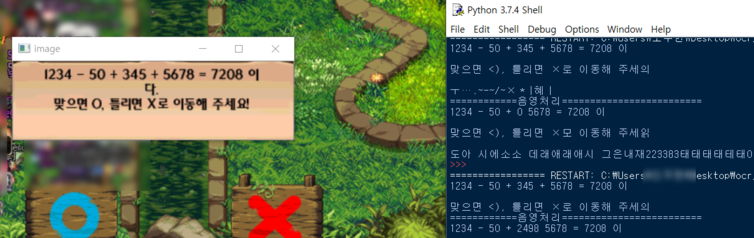
\includegraphics[width=\textwidth]{Figures/maplestory.png}
  \caption{%
    Example of an OCR engine reading \textit{hangeul} text
  }
  \label{fig:maplestory}
\end{figure}

Besides, this app aims to fulfill a niche as a cross-language ingredient scanner. The most popular commercial applications that already scan products and provide nutritional information, such as \textit{Yuka} \cite{noauthor_yuka_nodate-1} or \textit{MyRealFood} \cite{sl_myrealfood_nodate}, often do not provide the detailed ingredients list and most importantly, will not recognize products sold outside of their target region. They are also oriented towards providing nutritional scores based on food additives and cater to an audience interested in the \textit{real food}\footnote{Denomination given to foods that are not manufactured by processing and that do not contain food additives.} lifestyle, rather than being suited for people dealing with food intolerances.

On the other hand, while translators can perform accurately when reading Latin script, they often underperform when needing to recognize \textit{hangeul} script or when facing lists with complex terms instead of more structured text. As such, the most fundamental goal of the app is to be able to provide accurate readings of ingredients in Korean language and present the information and alerts to the user in a clean and streamlined manner.

\section{Objectives}

The prime objective of this DFP is the production of a fully functional mobile app, which will require the implementation and coordination of an ensemble of existing technologies, techniques and frameworks.

In order to compose said application, the following subobjectives will need to be materialized:

\begin{itemize}
\item Collection and study of prior bibliography, analysis of the existing solutions and approaches to similar problems implemented by other authors and identification of any potential new requirements.
\item Selection and installation of the technologies and tools that will be needed through the development process, formation in said technologies.
\item Recognition of the text on the product label. From a photograph, usage of any sort of preprocessing \cite{noauthor_optical_2021} and character recognition \cite{islam_survey_2016} tools and techniques needed to obtain the raw text.
\item Analysis of the output text, identifying the different ingredients, implementing any post-processing methods if needed (tokenization, segmentation, dictionary correction, etc.) \cite{kargin_nlp_2021} and matching with database.
\item Translation of the output text to be used as a fallback resource for unrecognized terms, implementing both on-device translation as well as a translation service API.
\item Finding an adequate data source and construction of a database architecture that stores the set of ingredients and possible synonyms to detect for each user profile or dietary need.
\item Development of the frontend of the application with a simple and usable interface intended for Android mobile devices. The application will allow the user to enter the unwanted ingredients, capture the images of the packaging and will return the list of ingredients in English along with an alert if it detects any specified allergens.
\end{itemize}

The proposed architecture for the mobile application, upon completion of this objectives and accounting with the technologies finally chosen, is the one shown in Figure \ref{fig:architecture}.

\begin{figure}[h]
  \centering
  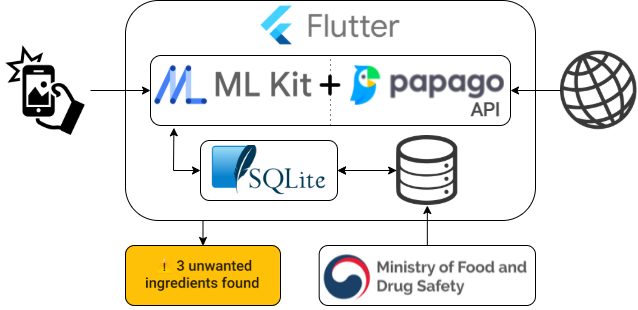
\includegraphics[width=\textwidth]{Figures/architecture.png}
  \caption{%
    Architecture of the mobile application
  }
  \label{fig:architecture}
\end{figure}

\section{Structure of this thesis}

In Chapter \ref{chapter1} we have introduced the main idea of our project, providing the adequate context to motivate and justify the topic for this thesis, as well as outlining the main goals and objectives that are expected to be met during its development.

Chapter \ref{chapter2} presents a compilation of previous works that tackle the same problem taken from the literature as well as including some commercial applications.

Through Chapter \ref{chapter3}, the planned schedule for the project is presented, defining in more detail the different tasks and subtasks that have been completed using a Gantt diagram. The time distribution is also discussed, justifying the varying amount of work hours allocated to each different task.

After it, Chapter \ref{chapter4} describes the software development methodology used through the work, presenting any relevant workflows or organization techniques used through the process.

The tools and technologies utilized for the completion of this project are detailed in Chapter \ref{chapter5}, providing a description about each of them and justifying the choice above other similar solutions.

Chapter \ref{chapter6} goes in detail through the whole development process, explaining every step of the implementation and reporting every problem encountered as well as the solutions that were found to overcome them.

In Chapter \ref{chapter7}, the results of the project are shown through practical examples and use cases to test the application behaviour and accuracy.

Finally, Chapter \ref{chapter8} presents the conclusions and lessons learned after the completion of the project, as well as introducing some other potential ideas for further iterations of the mobile application.
    \chapter{State of the art}
\label{chapter2}

Over the last few years, the main idea of this project has been broadly discussed and developed by other researchers. As such, there has been several projects that aimed to provide ingredient scanning tools for allergy patients on the literature. However, the popularity of user-ready applications that successfully implement this concept is reduced, as the few apps that have had a surge in popularity do not work nearly as well when dealing with food allergies. There is, however, some niche applications that effectively managed to implement a solution suited for patients of food intolerance.

In this chapter, we will select and discuss some of this projects, both from academic sources as well as commercial solutions freely available on app store platforms, in order to build a general picture about some of the recent developments made on this field.

\section{Literature review}

The central concept for this mobile application idea, text recognition over an ingredients list, has already been explored to some extent by previous authors, using different approaches which will serve as the foundation for the development of the application. On the following section two recent papers (from 2020 and 2021) that addressed the same problem will be discussed. The goal is to draw a comparison and highlight the differences between their proposed solution and the one intended for development during this project.

\subsection{Kamis and Shin}

Kamis and Shin \cite{putri_kamis_ocr-based_2020} used a similar approach to the intended in this project, performing OCR over the ingredients list in the package and refining this result using NLP techniques. Despite the recency of this paper, it provides a very robust framework in its solution that may be suited for all sort of similar applications. An adaptation of the implementation proposed in this paper, which also served as an initial guideline for this project, is shown in Figure \ref{fig:kamis}.

\begin{figure}[h]
  \centering
  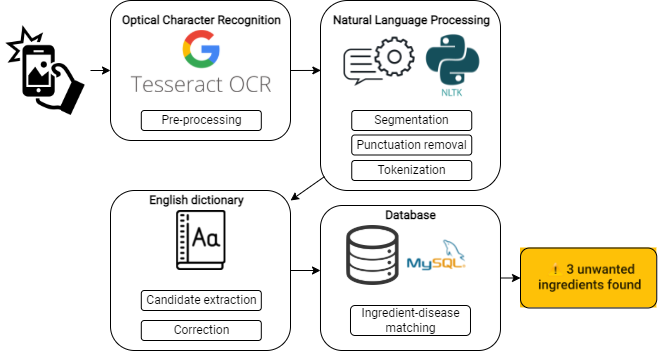
\includegraphics[width=\textwidth]{Figures/kamis.png}
  \caption{%
    Implementation schema proposed by Kamis and Shin
  }
  \label{fig:kamis}
\end{figure}

The one main difference is that this paper is designed entirely to work with English language and Latin script. Our project aims, however, to be used on Korean sources, which limits the range and effectiveness of OCR solutions available. \textit{Hangeul} text recognition is less trivial and systems are usually less refined and accurate for this script, which heavily deviates from the ubiquitous Latin script. In the same way, the array of data sources and processing tools is also more limited when working with Korean language, so other solutions will need to be found. Finally, the language barrier between the user and the input will also need to be addressed using a predefined database as well as an automated translation service.

\subsection{Jacky and Ma'muriyah}

Jacky and Ma'muriyah \cite{mamuriyah_perancangan_2021} have also developed a variation of this project, where the input taken is just the name of the food or dish and the ingredients are retrieved from a database. Other works from Korean authors \cite{lee_development_2017,yoon_web-app_2021} have taken the same approach to solving the problem. In this paper the developed application works over both \textit{hangeul} food names as well as romanized ones, although the accuracy achieved is higher when working with the latter. In Figure \ref{fig:kamis} we can see a practical example of their application correctly reading the name of a traditional Korean dish.

\begin{figure}[h]
  \centering
  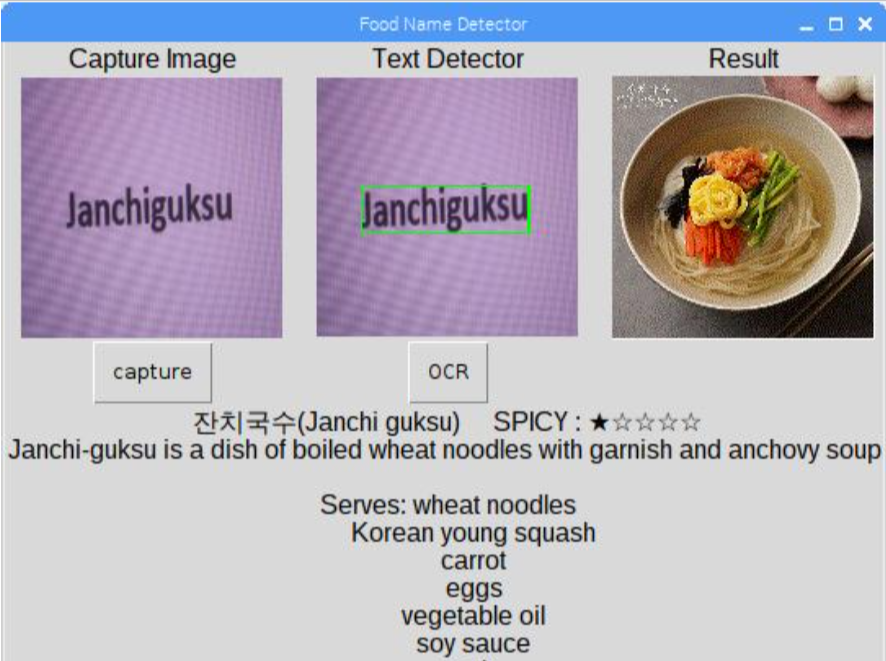
\includegraphics[width=0.5\textwidth]{Figures/jacky.png}
  \caption{%
    Execution example of the app developed by Jacky and Ma'muriyah
  }
  \label{fig:jacky}
\end{figure}

The main difference is that the project defined in this DFP aims to directly retrieve the ingredient list independent of the specific name of the product, so as to eliminate the need of maintaining an ever-changing database. This ensures that the application should work even on the newest of food products, as long as the ingredient list is humanly readable.

\section{Similar applications}

On this section, we will discuss some applications based on ideas that are similar to the subject of this project, detail its main features and compare them to the ones that our application implements.

\subsection{Yuka}

It should be noted that \textit{Yuka} \cite{noauthor_yuka_nodate-1} is not advertised as a food allergy-oriented ingredient scanner, and is more of a quality index provider for food products based on their added additives and nutritional information. However, given its huge popularity with more than 10 million downloads and 75.000 ratings \cite{noauthor_yuka_nodate} (which represents figures a thousand times higher than other apps in this section), it is included in this compilation. Its logotype is shown in Figure \ref{fig:yuka}.

\begin{figure}[h]
  \centering
  
\includegraphics[width=0.5\textwidth]{Figures/yuka.png}
  \caption{%
    Yuka's logotype
  }
  \label{fig:yuka}
\end{figure}

Despite not being specifically a scanner for food intolerances, it is capable of presenting the ingredients list for some of the items on their databases, and even supports new additions by taking a picture of the ingredients list. However, their OCR system does not support Korean language, therefore it is currently impossible to register products with packaging in Korean or attempt to scan their ingredients. For the products where it does work, there is no option present to set an alert in case a determinate ingredient is found, so the user should read and scan through the list manually. Some screenshots of the app interface can be seen on Figure \ref{fig:yuka-screenshot}.

\begin{figure}[h]
    \centering
    \begin{subfigure}{0.3\textwidth}
        \centering
        \includegraphics[width=0.9\linewidth]{Figures/Yuka-1.jpg}
        \caption{}
        \label{fig:yuka-1}
    \end{subfigure}
    \begin{subfigure}{0.3\textwidth}
        \centering
        \includegraphics[width=0.9\linewidth]{Figures/Yuka-2.jpg}
        \caption{}
        \label{fig:yuka-2}
    \end{subfigure}
    \begin{subfigure}{0.3\textwidth}
        \centering
        \includegraphics[width=0.9\linewidth]{Figures/Yuka-3.jpg}
        \caption{}
        \label{fig:yuka-3}
    \end{subfigure}
    \caption{Yuka app screenshots}
    \label{fig:yuka-screenshot}
\end{figure}

It supports barcode scanning as the main method for recognizing a product, with a prompt for OCR scanning if it has not been registered in their database yet. Because of this, the app will logically not function if the device is not connected to the Internet. On the UI aspect, \textit{Yuka} has a very clean and simple interface which will serve as inspiration for our mobile application.

\subsection{Soosee}

\textit{Soosee} \cite{noauthor_soosee_nodate-1} is a food scanner app specially developed for people with food allergies or intolerances. Its interface and functioning is quite simplified, with only three differentiated screens. On the second screen you can toggle which ingredients you want to detect, while on the main screen the detected allergens will appear highlighted on real time. Its logotype is shown in Figure \ref{fig:soosee}.

\begin{figure}[h]
  \centering
  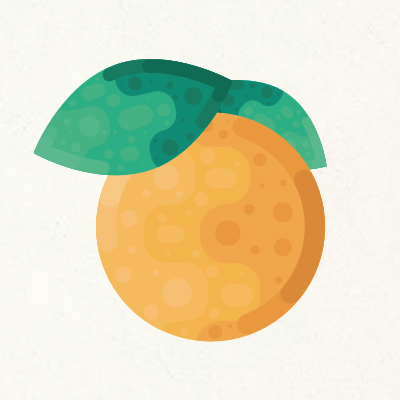
\includegraphics[width=0.25\textwidth]{Figures/soosee.png}
  \caption{%
    Soosee's logotype
  }
  \label{fig:soosee}
\end{figure}

Although this app is nearly not as popular as \textit{Yuka}, with around 10.000 total installs \cite{noauthor_soosee_nodate}, it is much more similar in its way of functioning to our target app. The main differences are that \textit{Soosee} does not support Korean language and that it does not support adding new ingredients, having only the option to toggle the existing ones. On the other hand, it features real-time scanning, which is a feature left out of the scope of our app. The main screens of \textit{Soosee} are shown on the screenshots in Figure \ref{fig:soosee-screenshot}.

\begin{figure}[h]
    \centering
    \begin{subfigure}{0.3\textwidth}
        \centering
        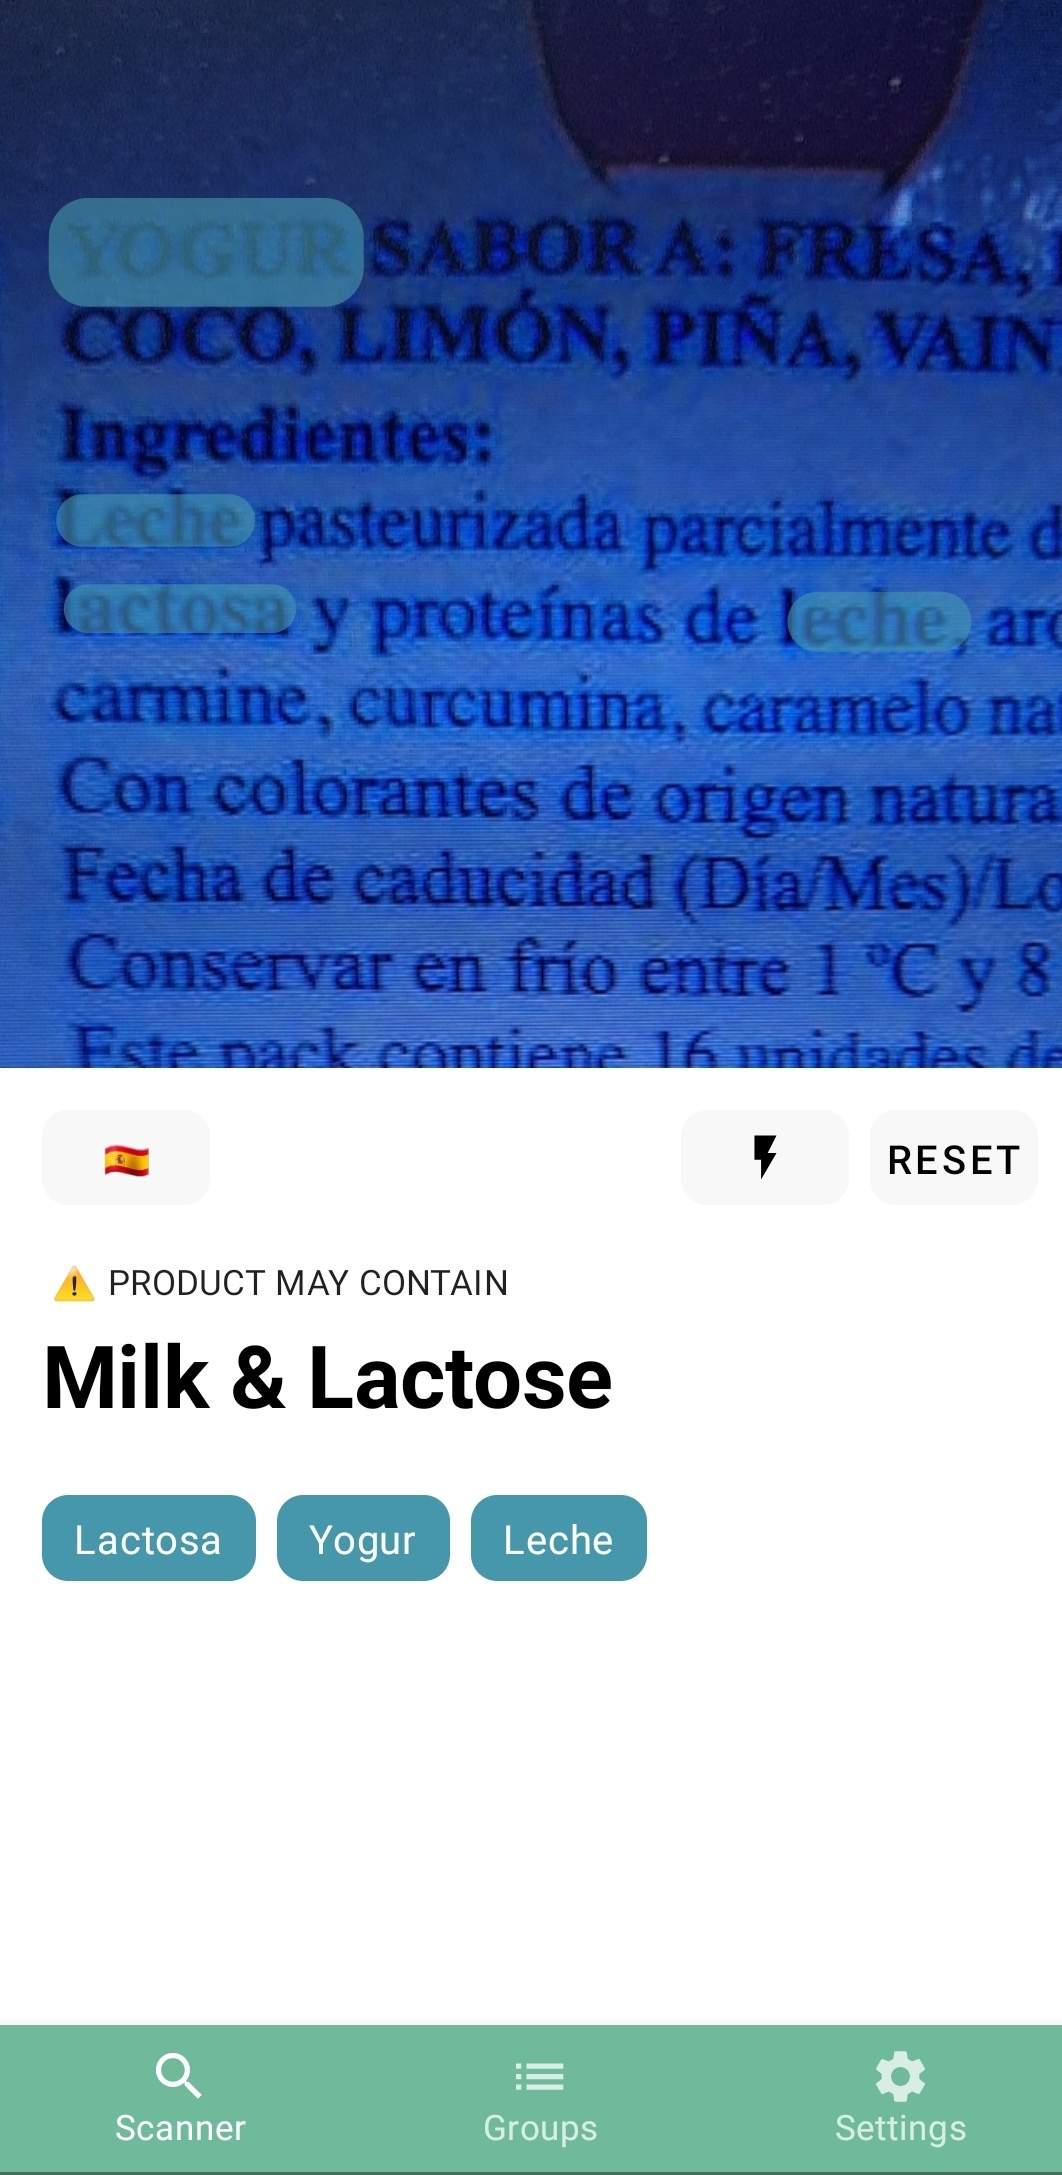
\includegraphics[width=0.9\linewidth]{Figures/soosee-1.jpg}
        \caption{}
        \label{fig:yuka-1}
    \end{subfigure}
    \begin{subfigure}{0.3\textwidth}
        \centering
        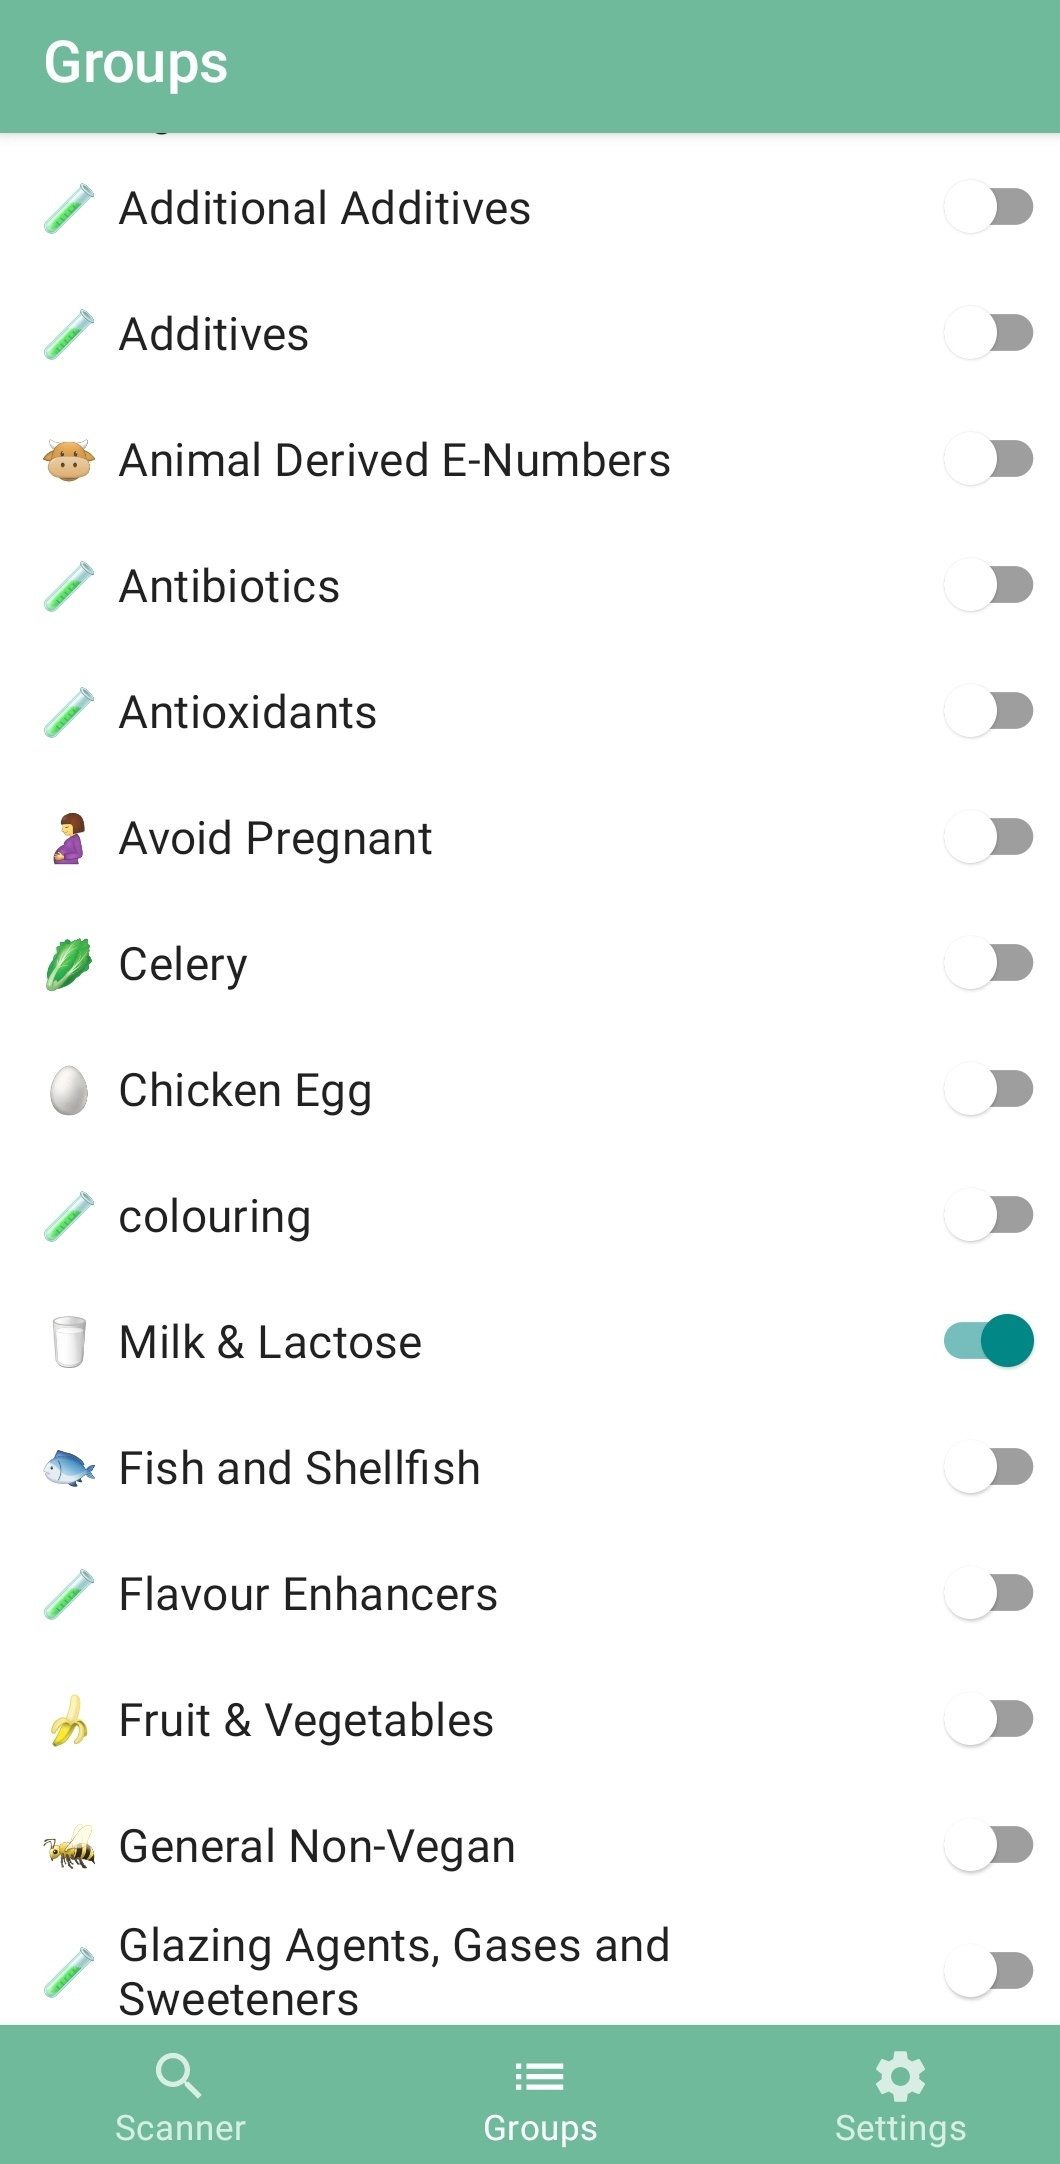
\includegraphics[width=0.9\linewidth]{Figures/soosee-2.jpg}
        \caption{}
        \label{fig:soosee-2}
    \end{subfigure}
    \begin{subfigure}{0.3\textwidth}
        \centering
        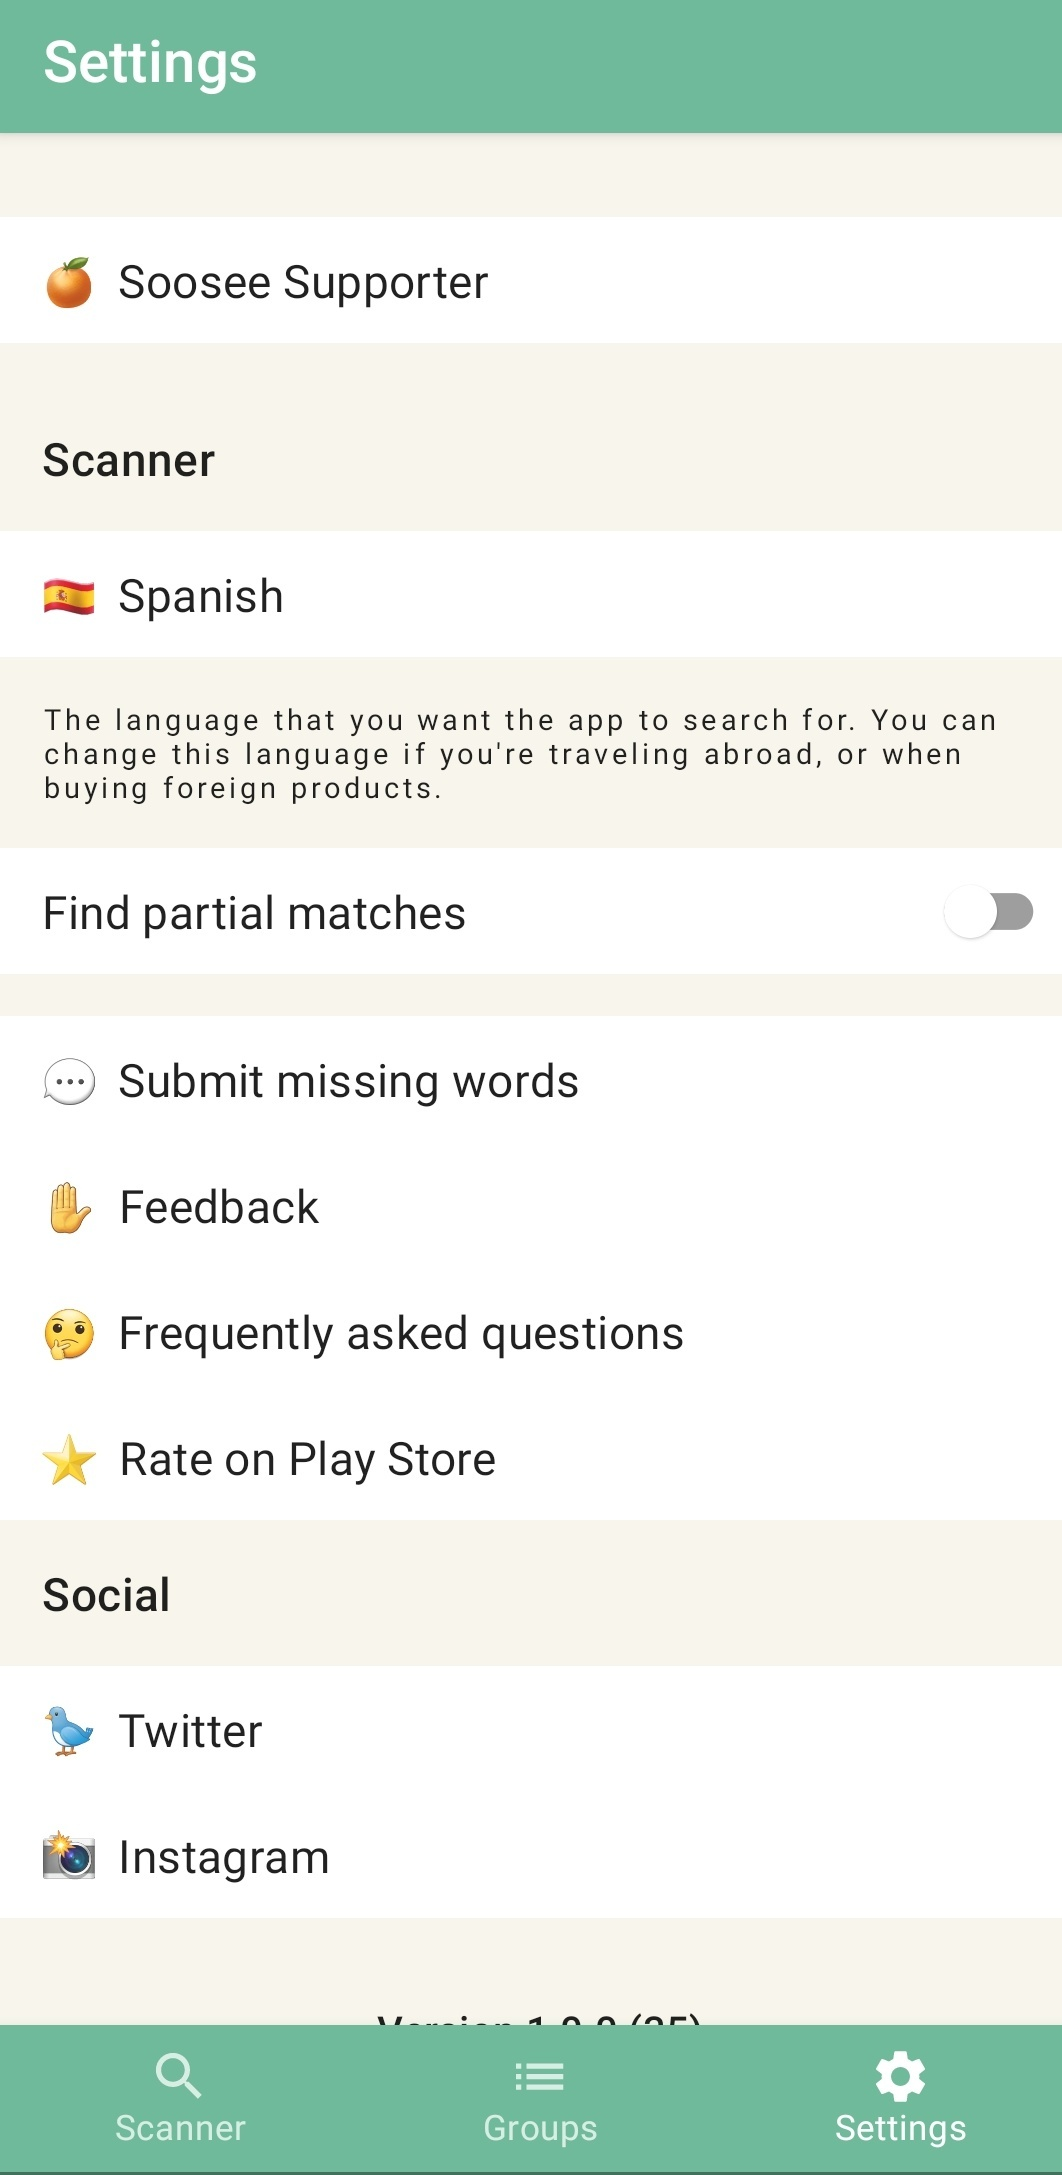
\includegraphics[width=0.9\linewidth]{Figures/soosee-3.jpg}
        \caption{}
        \label{fig:soosee-3}
    \end{subfigure}
    \caption{Soosee app screenshots}
    \label{fig:soosee-screenshot}
\end{figure}

\section{Feature comparison}

In Table \ref{tab:comparison}, we can see a summary of the comparison made on the previous sections. This table aims to include and compare those features that are more desirable for a user with food intolerances that primarily needs Korean support, English output and alerts when specific ingredients are found.

Under these assumptions, we can conclude that our app is the best choice for a user with these needs, supporting up to 6 features out of the 8 that were studied.
 
\begin{table}[h]
\centering
\begin{tabular}{@{}lccccc@{}}
\toprule
\textbf{}               & \textbf{Kamis et al.} & \textbf{Jacky et al.} & \textbf{Yuka} & \textbf{Soosee} & \textbf{Ours} \\ \midrule
Scanning of Korean text & -                     & \checkmark            & -             & -               & \checkmark    \\
Translation             & -                     & -                     & -             & -               & \checkmark    \\
Search history          & -                     & -                     & \checkmark    & -               & \checkmark    \\
Custom ingredients      & -                     & -                     & -             & \checkmark      & \checkmark    \\
Ingredient alerts       & \checkmark            & -                     & -             & \checkmark      & \checkmark    \\
Cross-language          & -                     & \checkmark            & \checkmark    & \checkmark      & \checkmark    \\
Barcode scanning        & -                     & -                     & \checkmark    & -               & -             \\
Real-time results       & -                     & -                     & -             & \checkmark      & -             \\ \bottomrule
\end{tabular}
\caption{%
    Feature comparison across all alternatives
}
\label{tab:comparison}
\end{table}
    \chapter{Development phases}
\label{chapter3}

In this chapter, we introduce the division and scheduling of every process that needs to be carried out in order to complete the project that is presented in this DFP. A Gantt chart is provided describing the actual time allocated to each of the tasks, as well as some additional graphs and charts presenting other details of the followed schedule.

\section{Gantt chart}

Since the original planning, the total work to be done had been organized into the \textit{6 development phases}, each of them as well divided into a set of subprocesses, that are detailed in the Gantt chart in Figure \ref{fig:gantt}.

\begin{figure}[h]
  \centering
  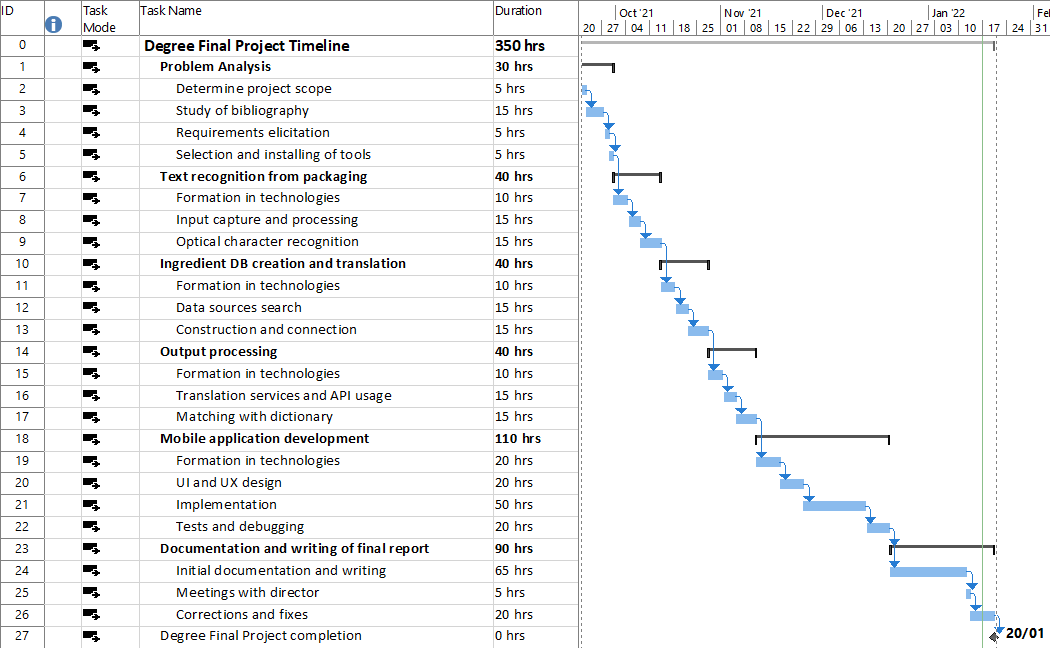
\includegraphics[width=\textwidth]{Figures/gantt.png}
  \caption{%
    Gantt chart for the development of the DFP
  }
  \label{fig:gantt}
\end{figure}

The timing had originally been estimated for work days of 20 hours per week, adding to a total of \textit{300 hours} of work over \textit{15 weeks}. While this calculation was made according to the DFP guidelines, it ended up underestimating the actual time that some of the processes took to complete, such as the time designated to the implementation and coding of the app or to the writing of this document. With these adjustments, the total time dedicated was approximately \textit{350 hours} of work, executed over \textit{17.5 weeks} or roughly 4 months.

An extended version of this Gantt chart (Figure \ref{fig:gantt_actual}), as well as the Gantt chart used in the original planning (Figure \ref{fig:gantt_planned}) for comparison reference, are available on appendix \ref{appendix:A}.

\subsection{Timeline}

In Figure \ref{fig:timeline}, we can see the timeline view of the project with the start and ending dates for each of the milestones. As the development followed a sequential approach, there was no overlapping between any of the processes and each of them was started only as the previous one finished. The initial four tasks spanned over the first two months of development, while another two months were dedicated to the two final tasks.

\begin{figure}[h]
  \centering
  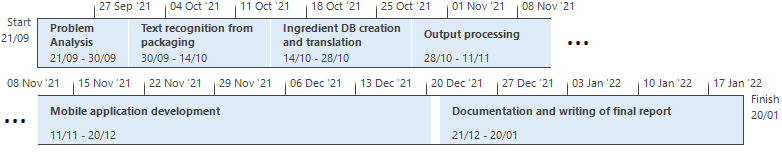
\includegraphics[width=\textwidth]{Figures/timeline.png}
  \caption{%
    Timeline for the development of the DFP
  }
  \label{fig:timeline}
\end{figure}

\section{Time distribution}

As shown in Figure \ref{fig:ganttbars}, the time distribution across all of the 6 processes was quite uneven, with some of the tasks demanding almost twice as much time as others. In particular, the coding and implementation of the app, as well as the writing of this report, took more time than all of the remaining tasks combined.

On the other hand, prior tasks were shorter in time and had more straightforward subobjectives that would be used at later stages. This subobjectives would later be put together to compose the mobile application on the development stage.

\begin{figure}[h]
  \centering
  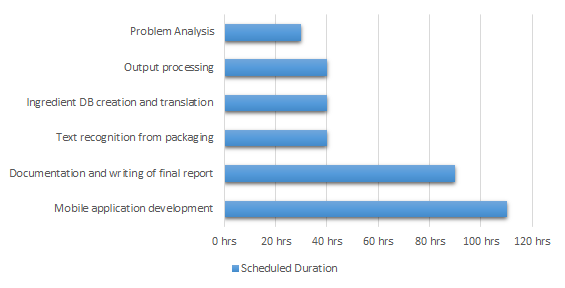
\includegraphics[width=\textwidth]{Figures/ganttbars.png}
  \caption{%
    Distribution of hours per development phase
  }
  \label{fig:ganttbars}
\end{figure}

This distribution was expected since the first tasks, without being any less relevant than the last, were focused on studying the literature and finding the right approach for the project. While some actual construction of the app was done at this steps, such as collecting and organizing the source data in a database or doing preliminary tests for the OCR implementation, most of the development was condensed on the last stages.
    \chapter{Methodology}
\label{chapter4}

In Chapter \ref{chapter4}, we will define and elaborate on the software development methodology that was followed through the different processes of this project. We will also explain other workflows that complemented this methodology such as the usage of version control and a Kanban board for issue tracking and backlogging of features and fixes.

\section{Waterfall}

On the initial planning, the development methodology that was designated to be used through our project was be an iterative or waterfall model \cite{balaji_waterfall_2012}, since it seemed clear that each phase had to be completed before starting the next and no work was planned in parallel. Development would then be organized following the schema in Figure \ref{fig:waterfall} \cite{noauthor__2021}.

\begin{figure}[h]
  \centering
  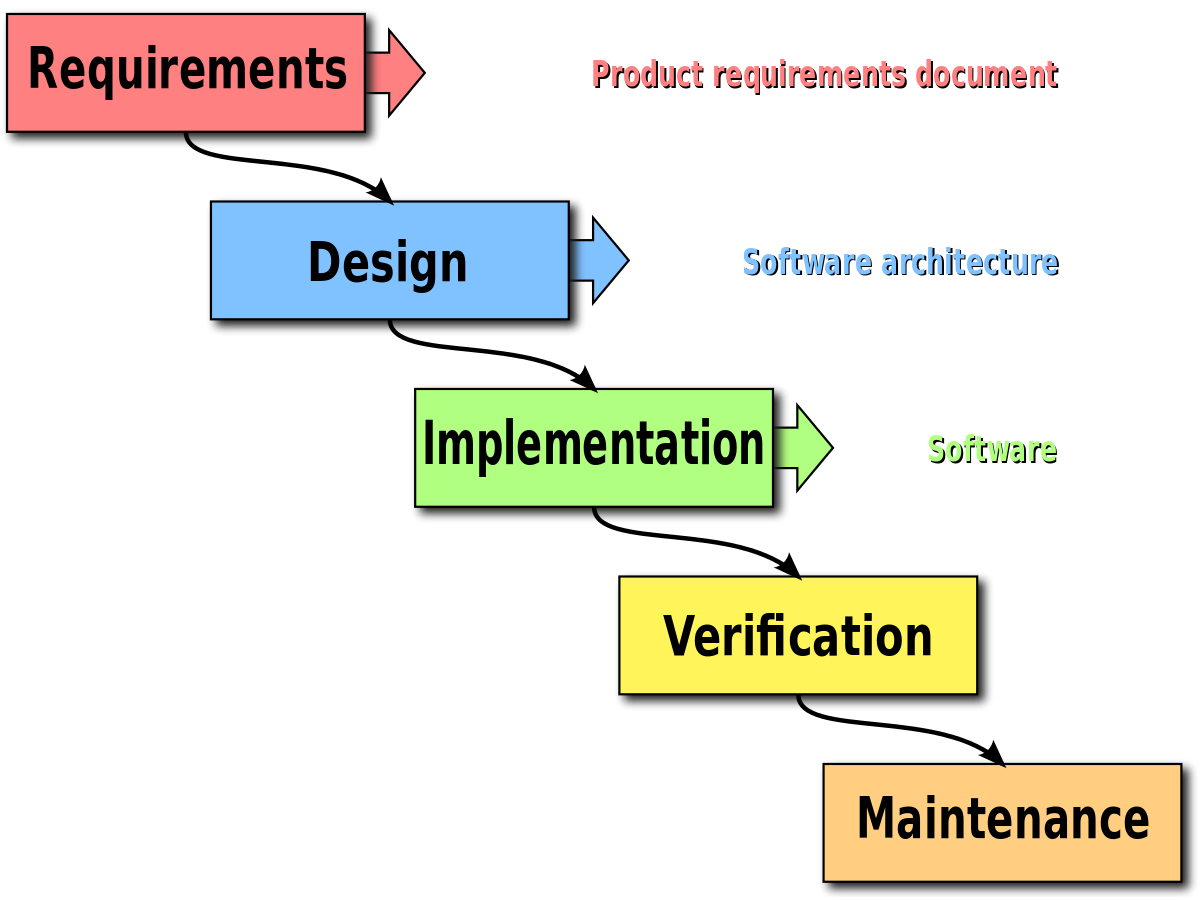
\includegraphics[width=0.6\textwidth]{Figures/waterfall.png}
  \caption{%
    Waterfall methodology base schema
  }
  \label{fig:waterfall}
\end{figure}

However, shortly upon the start of the project, it was clear that this was not the ideal methodology to follow. While the main intention was to complete every stage in a sequential manner, we often found the need to go back to iterate on what had already been completed in order to achieve a better solution.

Therefore, it was decided that as the project was going to be developed by a single person, certain flexibility should be adopted by adding some elements from agile methodologies. In this way elements from \textit{scrum} were quickly incorporated into the workflow, such as periodic meetings with the tutor along with the possible revisions of the requirements.

\section{Scrum}

\textit{Scrum} \cite{noauthor_scrum_2022} is an agile methodology for software development designed for small teams, where the final product is broken into several subobjectives to be completed through several \textit{sprints}. These \textit{sprints} are timed iterations of the final product, each of them taking typically around two weeks to complete. The Figure \ref{fig:scrum} shows the main framework for a \textit{scrum} project. 

\begin{figure}[h]
  \centering
  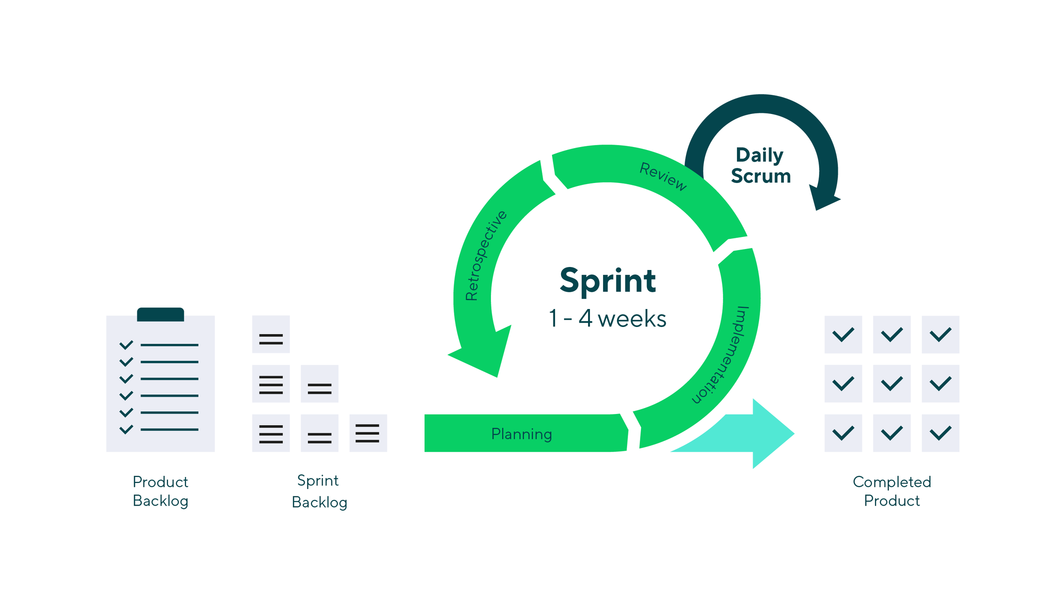
\includegraphics[width=\textwidth]{Figures/scrum.png}
  \caption{%
    Scrum methodology base schema
  }
  \label{fig:scrum}
\end{figure}

We can see each \textit{sprint} is composed of a Sprint Backlog, whose elements are at the same time a subset of objectives taken for a Product Backlog. This Product Backlog is a list containing each and every objective that needs to be materialized in order to compose the finished project. The elements taken from the Product Backlog for each \textit{sprint} are usually chosen considering the best ratio between the time required and the importance or satisfaction for the client.

In the particular case of this project, Sprint Backlogs were not formally defined, as the timezone difference and other incompatibilities made it difficult to have frequent and fixed in time meetings with the Scrum Master (the DFP director in this case) which delimit and determine the contents of each \textit{sprint}.

However, a Product Backlog was established and several deadlines were defined in order to ensure that the development progressed according to the schedule. The most crucial items were selected from the Product Backlog in each iteration according to the criteria of the developer. This Product Backlog was implemented into the workflow by using a Kanban board.

\section{Kanban}

Kanban \cite{noauthor_kanban_2021} is a framework or methodology for software development which is centered around a Kanban board. In a Kanban board, tasks are presented as cards and distributed across several columns, usually representing the possible stages of development for every job. 

In our project, we utilized a Kanban board as an organization tool for keeping track of both issues and proposed features. Using GitHub projects \cite{noauthor_githubcom_2021}, we can automate the board so as to automatically move the tasks as we mark as solved the issues associated. The Kanban board for the project can be seen in Figure \ref{fig:kanban}, and it can also be found in its corresponding GitHub repository\footnote{Available at: \url{github.com/dogudo/tfg}}.

\begin{figure}[h]
  \centering
  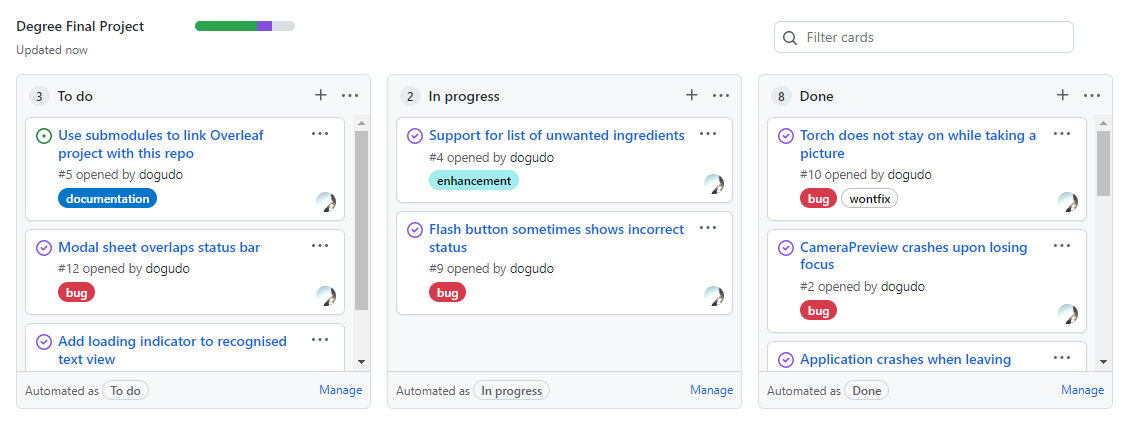
\includegraphics[width=\textwidth]{Figures/kanban_board.png}
  \caption{%
    Kanban board
  }
  \label{fig:kanban}
\end{figure}

The issues that feed the Kanban board are created at the Issues section of the GitHub repository. In this tab we can create entries for any kind of issue or enhancement and associate some tags to them, such as \textit{bug}, \textit{feature}, \textit{documentation}, etc. We can also assign any user to the task (in this case all of the tasks are assigned to the repository owner) and allocate them to different milestones, which can function similar to the \textit{sprints} proposed in \textit{scrum} methodology. The issue tracker view is shown in Figure \ref{fig:issue-tracking}.

\begin{figure}[h]
  \centering
  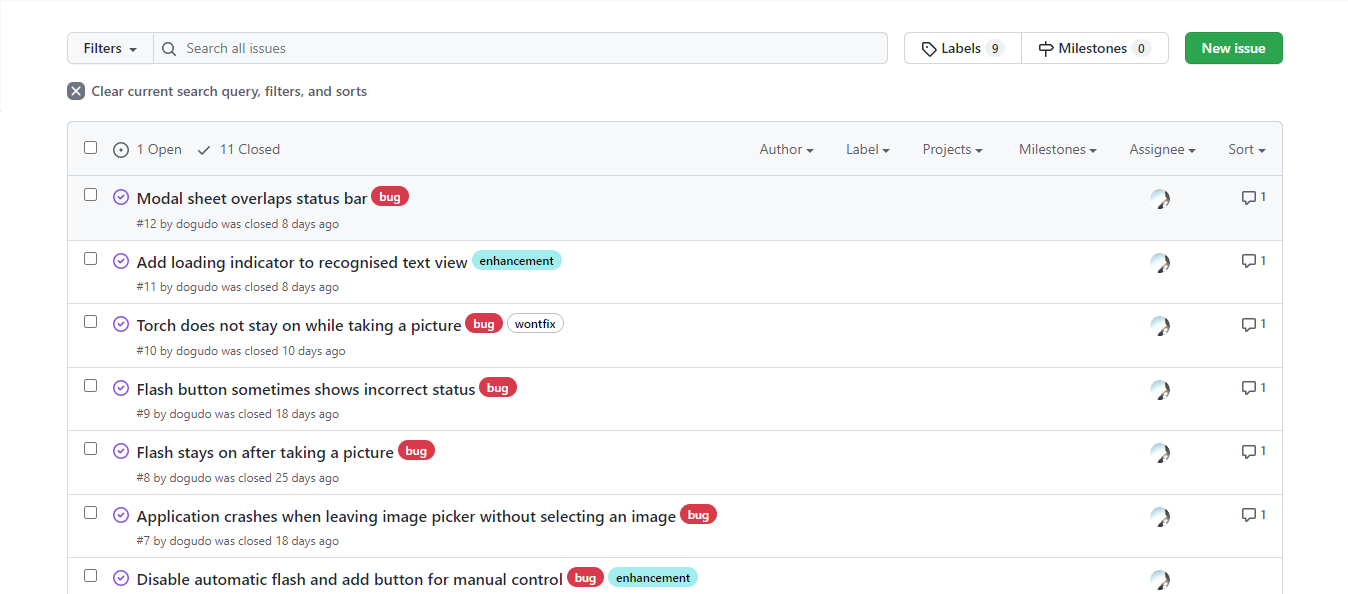
\includegraphics[width=\textwidth]{Figures/issue_tracking.png}
  \caption{%
    Issue tracking
  }
  \label{fig:issue-tracking}
\end{figure}

If we open any of this issues, a timeline view is shown we can add any type of comments to keep reference of the progress being made. Figure \ref{fig:timeline} depicts this timeline view for one of the issues, which has some comments, commits, and a Kanban card associated with it.

\begin{figure}[h]
  \centering
  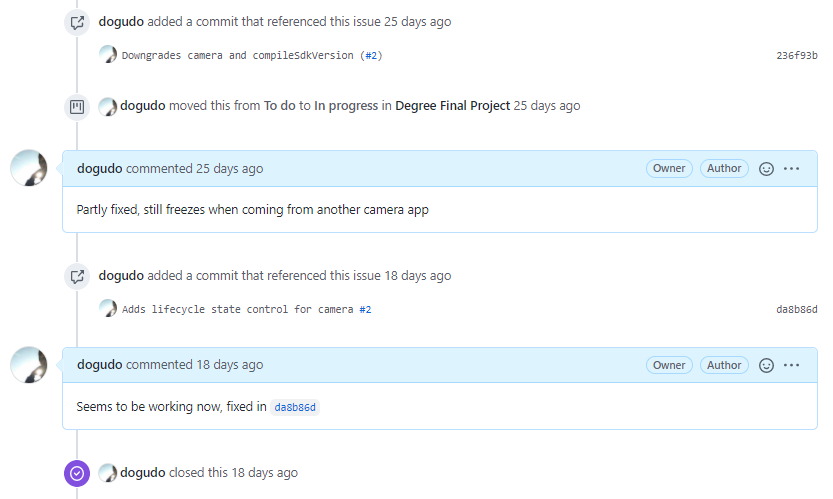
\includegraphics[width=0.8\textwidth]{Figures/issue_timeline.png}
  \caption{%
    Example of timeline view for an issue
  }
  \label{fig:issue-timeline}
\end{figure}

As mentioned before, we can also use the Milestones feature to associate a set of issues with a due date, therefore emulating the \textit{sprints} that characterize the \textit{scrum} methodology. Figure \ref{fig:milestones} shows two of the milestones that were defined for the project.

\begin{figure}[h]
  \centering
  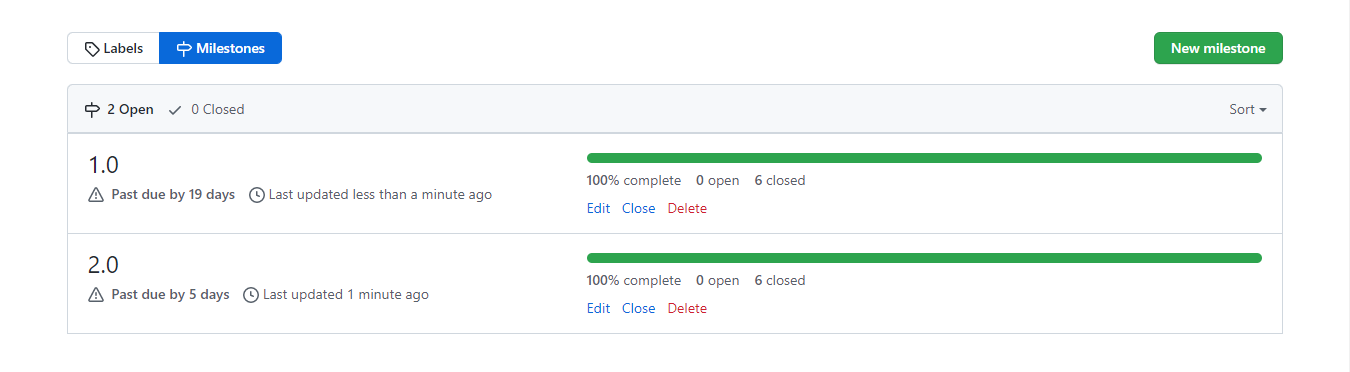
\includegraphics[width=\textwidth]{Figures/milestones.png}
  \caption{%
    Milestones for the project
  }
  \label{fig:milestones}
\end{figure}
    \chapter{Tools and technologies}
\label{chapter5}

In this chapter, we will thoroughly describe the tools, technologies and other materials that were utilized in any way to help in the development of this Degree Final Project. This includes any necessary programming languages, plugins, IDEs, APIs, database engines, data sources and any other software development and documentation tools that were needed at any stage of the process for building the mobile application.

Besides, for some of them we will also provide a comparison with other similar options and justify why it was finally decided to choose them for this project over the rest of available solutions. As a summary, the tools and technologies that were used to plan and develop the mobile application are the following:

\begin{itemize}
\item For building the Android mobile application we will make use of the open-source Flutter framework \cite{noauthor_flutter_2021}, which also supports a wide variety of plugins for OCR, database management, UI design, etc.
\item To capture the text, we will work with the ML Kit SDK \cite{noauthor_ml_nodate} which includes an optical character recognition model, also open-source, and with the Flutter plugin \texttt{google\_ml\_kit} \cite{noauthor_google_ml_kit_nodate}.
\item In the case of post-processing the text and translating any ingredients not included in the database, we will make use of the Papago API \cite{noauthor__nodate} provided by Naver.
\item The database will be created and maintained using the SQLite relational management system \cite{noauthor_sqlite_nodate}.
\item The development of all the code will be done using the Visual Studio Code text editor \cite{noauthor_documentation_2021}, as well as the Android Studio IDE \cite{noauthor_introduccion_2021}. The source code control will be done with Git \cite{noauthor_git_2021} and GitHub \cite{noauthor_githubcom_2021}.
\end{itemize}

\section{Framework}

In this section we will introduce and discuss the framework chosen to support the mobile application architecture, Flutter, going though some of its main characteristics. We will also detail the programming language it uses, Dart, as well as the most relevant Flutter plugins that were utilized during development.

\subsection{Flutter}

Flutter \cite{noauthor_flutter_2021} is an open-source framework for mobile applications development created by Google in 2017. It supports cross-platform development, allowing to generate Android, iOS and web apps from the same codebase. Its logotype is shown in Figure \ref{fig:flutter}.

\begin{figure}[h]
  \centering
  
\includegraphics[width=0.5\textwidth]{Figures/flutter.png}
  \caption{%
    Flutter's logotype
  }
  \label{fig:flutter}
\end{figure}

Its main characteristic is that all of the app design and architecture in Flutter is based on components called widgets. A widget in Flutter can be any description of part of a user infer face along with some data. We can combine several simple widgets to produce more complex ones, thus organizing all the interface design and behaviour in a hierarchical tree structure where every element is a widget. In Figure \ref{fig:flutter-widgets} we can see an example of this tree hierarchy for a simple app.

\begin{figure}[h]
  \centering
  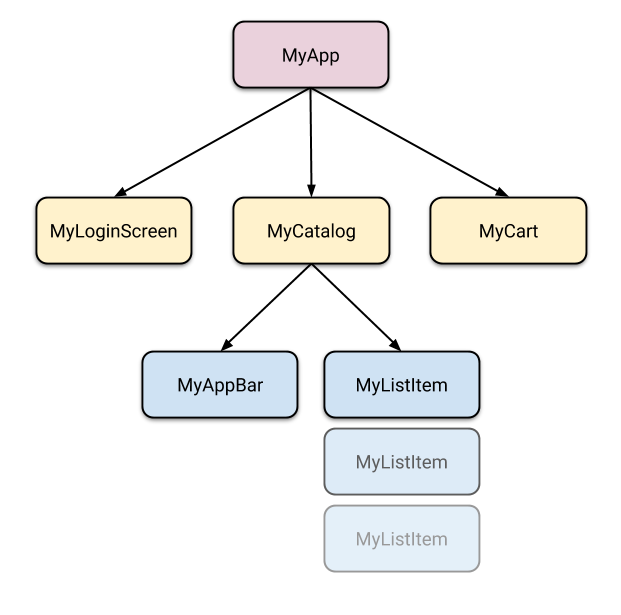
\includegraphics[width=0.5\textwidth]{Figures/flutter-widgets.png}
  \caption{%
    Tree of widgets that compose a Flutter app
  }
  \label{fig:flutter-widgets}
\end{figure}

Some of these widgets are already predesigned to conform to established design guidelines, such as Material Design \cite{noauthor_material_nodate} for Android or the Cupertino library for adhering to iOS style. In our application, we made extensive use of the Material library in order to keep a consistent design with other Android apps.

These support for visually clean components gave it an edge over other similar frameworks available for cross-platform development, such as React Native, Xamarin or Ionic. Other reasons for choosing Flutter are that its developed by the same company that maintains Android, Google, and that the community built around Flutter has gotten quite large over the recent years. In fact, during the development of this project, we managed to locate and solve several issues by contacting other Flutter developers via channels like GitHub or Discord.

An example of this communications can be seen in Figure \ref{fig:flutter-issue}, which shows an issue opened to fix a camera bug.

\begin{figure}[h]
  \centering
  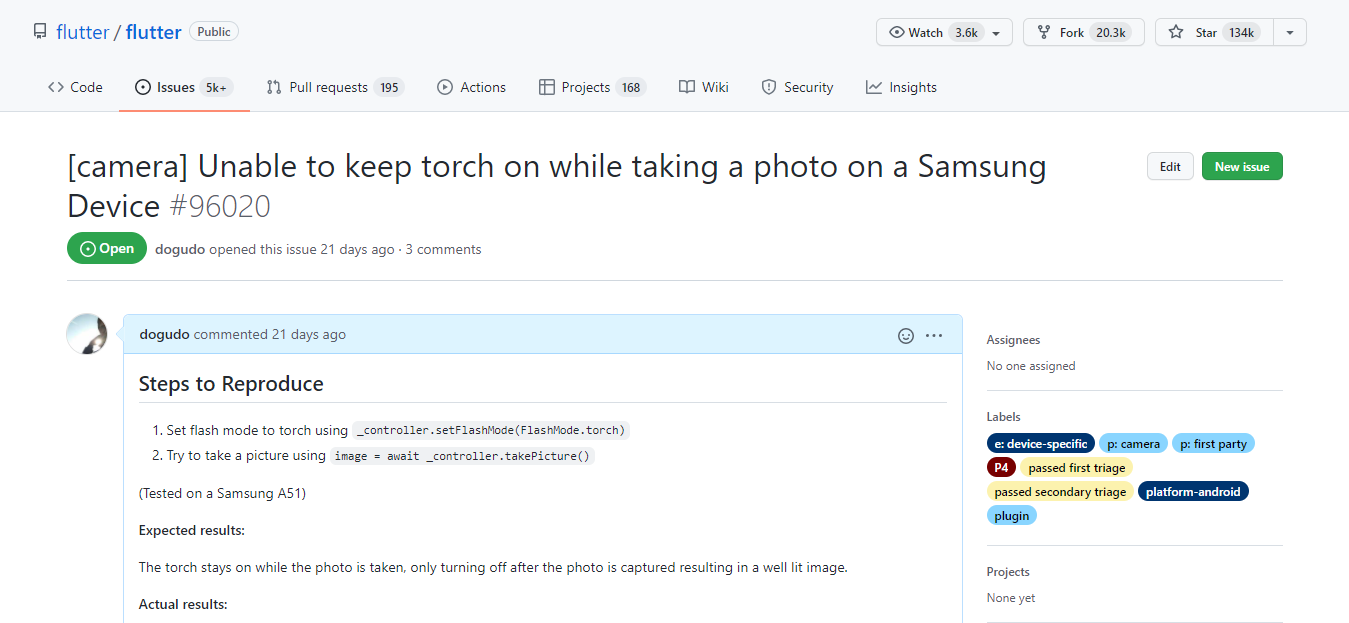
\includegraphics[width=\textwidth]{Figures/flutter-issue.png}
  \caption{%
    Issue opened in Flutter's issue tracker
  }
  \label{fig:flutter-issue}
\end{figure}

Lastly, the programming language that is utilized through all stages of Flutter's app development is Dart.

\subsection{Dart}

Dart \cite{noauthor_dart_nodate-1} is an open-source programming language developed by Google and specifically designed for web and mobile apps development. As it has been mentioned, it is Flutter's development language although it was first released in 2010. It is optimized for client-side development and one of its biggest strengths is capability to compile to either native code or JavaScript. This way, it is properly suited for cross-platform development. Its logotype can be seen in Figure \ref{fig:dart}.

\begin{figure}[h]
  \centering
  
\includegraphics[width=0.5\textwidth]{Figures/dart.png}
  \caption{%
    Dart's logotype
  }
  \label{fig:dart}
\end{figure}

Some of Dart's most relevant and differentiating characteristics from other languages are listed below:

\begin{itemize}
\item \textbf{Null safety}: by default, values in Dart cannot be null unless the developer explicitly specifies so.
\item \textbf{Strongly typed}: although type annotations are optional because they can be inferred by the compiler.
\item \textbf{Asynchronous programming}: supported by using futures as well as the \texttt{async} and \texttt{await} keywords. This is specially useful for interfaces, where some elements may need to wait for some other operation to finish before being displayed.
\end{itemize}

For quick reference of how a Dart code file actually looks like, a snippet from the application is provided on Listing \ref{lst:dart}.

\begin{code}
\begin{minted}
[
breaklines,
frame=lines,
framesep=2mm,
baselinestretch=1.2,
fontsize=\footnotesize,
linenos
]
{dart}
  Widget build(BuildContext context) {
    return AnnotatedRegion<SystemUiOverlayStyle>(
      child: Scaffold(
        appBar: AppBar(
          title: Text(widget.title),
          systemOverlayStyle: const SystemUiOverlayStyle(
            statusBarColor: Colors.transparent,
          ),
        ),
        body: Center(
          child: screens.elementAt(_selectedIndex),
        ),
        bottomNavigationBar: BottomNavigationBar(
          items: const <BottomNavigationBarItem>[
            BottomNavigationBarItem(
              icon: Icon(Icons.history),
              label: 'History',
            ),
            BottomNavigationBarItem(
              icon: Icon(Icons.home),
              label: 'Allergens',
            ),
          ],
          currentIndex: _selectedIndex,
          onTap: _onItemTapped,
        ),
      ),
    );
  }
\end{minted}
\caption{Example of Dart code}
\label{lst:dart}
\end{code}

\subsection{Plugins}

Flutter plugins or packages are libraries of code that expand the capabilities of the base framework. They are published in the package repository Pub \cite{noauthor_dart_nodate}, where developers can browse through a large collection of packages to easily incorporate other technologies, functionalities or APIs into their application. This repository's main page is seen in Figure \ref{fig:pub}.

\begin{figure}[h]
  \centering
  
\includegraphics[width=0.75\textwidth]{Figures/pub.png}
  \caption{%
    Pub's homepage snippet
  }
  \label{fig:pub}
\end{figure}

During the development of our application we had to incorporate up to seven new dependencies into our Flutter codebase. Some of the most interesting ones are listed below:

\begin{itemize}
\item \textbf{\texttt{google\_ml\_kit}} \cite{noauthor_google_ml_kit_nodate}: recently released plugin that provides an easy way to implement Google's standalone ML Kit in a Flutter app instead of on a native Android one. It will be broadly discussed on the next section.
\item \textbf{\texttt{camera}} \cite{noauthor_camera_nodate}: a plugin providing access and some control functionality over the device cameras. Used for a better integration with our UI than when using the device native camera app.
\item \textbf{\texttt{sqflite}} \cite{noauthor_sqflite_nodate}: a plugin providing support for operating the SQLite database engine through a Flutter app.
\item \textbf{\texttt{http}} \cite{noauthor_http_nodate}: a future-based library dedicated to make HTTP requests, used mainly for API requests.
\end{itemize}

\section{SDK and API}

This section will further explain two of the main technologies at the core of the mobile application, its text recognition system and its translation system, and justify the choice of these solutions.

\subsection{ML Kit}

Google ML Kit \cite{noauthor_ml_nodate} is a mobile SDK that provides on-device machine learning solutions to both Android and iOS apps. By default, only native Android apps are supported by this SDK. However, by using the \texttt{google\_ml\_kit} plugin previously mentioned, it is considerably simpler to make use of this technology on a Flutter application. ML Kit's logotype is shown in Figure \ref{fig:ml-kit}.

\begin{figure}[h]
  \centering
  
\includegraphics[width=0.5\textwidth]{Figures/ml-kit.png}
  \caption{%
    ML Kit's logotype.
  }
  \label{fig:ml-kit}
\end{figure}

Even though initially this technology did not support Korean language for its text recognition models, support for non-Latin scripts like \textit{hangeul} among others was added on a beta update released on August of 2021. This allows for accurate Korean text recognition without needing to incur on external API additional costs, since all the processing is done on-device. On the downside, the size of the application increases considerably, up to 400 MB.

In addition to this text recognition API, an on-device translation API is also provided. Due to its low accuracy this one is used only as a fallback for when the main one, the Papago API, is not available.

\subsection{Papago API}

Papago is a translation service developed by Naver, one of the companies leading the technology sector in South Korea. It is one of the most used translation services along with Google Translate, and supports up to 15 languages including Korean, English and Spanish. Its logo is shown in Figure \ref{fig:papago}.

\begin{figure}[h]
  \centering
  
\includegraphics[width=0.5\textwidth]{Figures/papago.png}
  \caption{%
    Papago's logotype.
  }
  \label{fig:papago}
\end{figure}

Fortunately, Naver provides a quite generous RESTful API service for Papago, providing free translations of up to 10000 characters per day when registering our application in their system. This limit can be seen on Figure \ref{fig:papago-limit} and is one of the main reasons for choosing this service, as Google Translate API is paid since the first query. One other relevant reason being that, in the author experience, Papago provides more accurate and consistent translations than other services when working between English and Korean languages.

\begin{figure}[h]
  \centering
  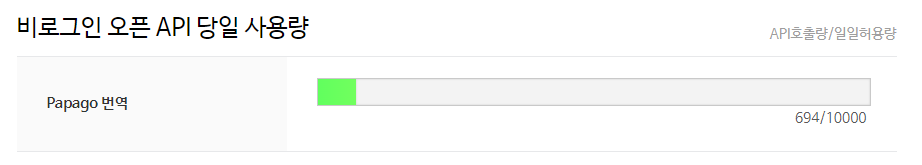
\includegraphics[width=\textwidth]{Figures/papago-limit.png}
  \caption{%
    Papago's API daily character limit.
  }
  \label{fig:papago-limit}
\end{figure}

\section{Database}

This section we will discuss the database engine utilized for the backend of this project. We will also introduce the tools that were used for the management of the databases, as well as explaining the source of the data that provides the list of ingredients, categories, etc.

\subsection{SQLite}

SQLite \cite{noauthor_sqlite_nodate} is a relational database engine which is contained on a small library written in C. It is one of the most used database engines in the world as it is cross-platform and relatively light and simple. Its logotype is shown in Figure \ref{fig:sqlite}.

\begin{figure}[h]
  \centering
  
\includegraphics[width=0.5\textwidth]{Figures/sqlite.png}
  \caption{%
    SQLite's logotype.
  }
  \label{fig:sqlite}
\end{figure}

The main difference between SQLite and other database engines is that SQLite is not an independent process from the application that it supports. Instead, the SQLite library is directly linked with the code of the application, as opposed to other systems and engines that maintain a client-server structure. The diagram in Figure \ref{fig:sqlite-architecture} provides a comprehensible overview of the differences in the architecture.

\begin{figure}[h]
  \centering
  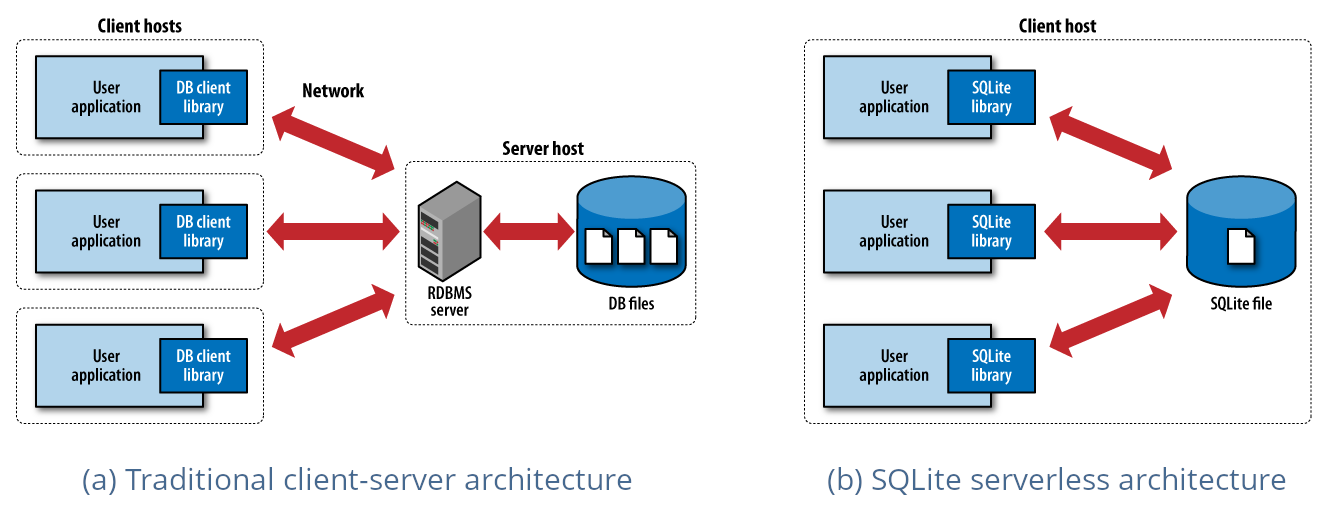
\includegraphics[width=\textwidth]{Figures/sqlite-architecture.png}
  \caption{%
    Comparison between SQLite and traditional client-server
  }
  \label{fig:sqlite-architecture}
\end{figure}

This is one of the main reasons for choosing SQLite for this project and why it is so popular for other Flutter projects, since we only need a small and user dependent database with few tables that also supports offline access.

\subsection{DB Browser for SQLite}

DB Browser for SQLite \cite{noauthor_db_nodate}, abbreviated DB4S, is a GUI client for browsing and modifying database files compatible with SQLite. It uses a spreadsheet-like interface as most other GUI database editors, and provides several shortcuts for some of the most common SQLite commands. Its logotype is shown in Figure \ref{fig:db4s}.

\begin{figure}[h]
  \centering
  
\includegraphics[width=0.25\textwidth]{Figures/db4s.png}
  \caption{%
    DB Browser for SQLite's logotype
  }
  \label{fig:db4s}
\end{figure}

We made use of this tool because we needed to manually edit some of the data obtained from the data sources listed in the next section. Though this is doable on a CLI interface, it is certainly much more inconvenient and time consuming for finicky tasks like this one. We can have a look at DB Browser for SQLite's interface in Figure \ref{fig:db4s-screen}.

\begin{figure}[h]
  \centering
  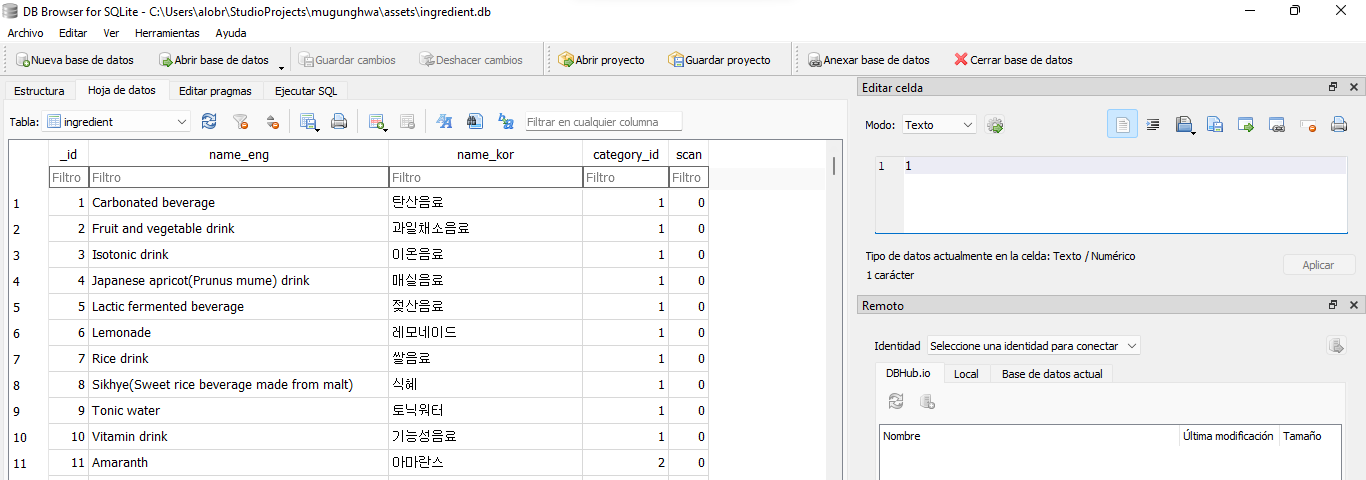
\includegraphics[width=\textwidth]{Figures/db4s-screen.png}
  \caption{%
    DB Browser for SQLite's user interface
  }
  \label{fig:db4s-screen}
\end{figure}

\subsection{Data source}

In order to develop the backend of the application we need a pre-made list of one of the ingredients most commonly used in Korea as well as their translations to English. This data source was eventually found in the Food Safety Korea portal \cite{noauthor__nodate-1}, an organism dependent of the Ministry of Food and Drug safety of South Korea. A screenshot of this website is shown in Figure \ref{fig:fsk}.

\begin{figure}[h]
  \centering
  
\includegraphics[width=\textwidth]{Figures/fsk.png}
  \caption{%
    Screenshot of the Food Safety Korea website
  }
  \label{fig:fsk}
\end{figure}

This website is a portal which offers direct access to several search engines, APIs and databases to collect every possible data source related to food safety in South Korea. Among all of these sources we chose the Food Composition Database search \cite{noauthor_food_nodate}, which is also listed in the Food and Agriculture Organization (FAO) of the UN as the reference for ingredients list in Korea.

After filing a small questionnaire this dataset was provided as an Excel spreadsheet, which needed to be cleaned out of redundant entries and converted to a CSV file in order to be imported into a table in our database using DB Browser for SQLite. The initial Excel file had the appearance shown in Figure \ref{fig:fsk-data}.

\begin{figure}[h]
  \centering
  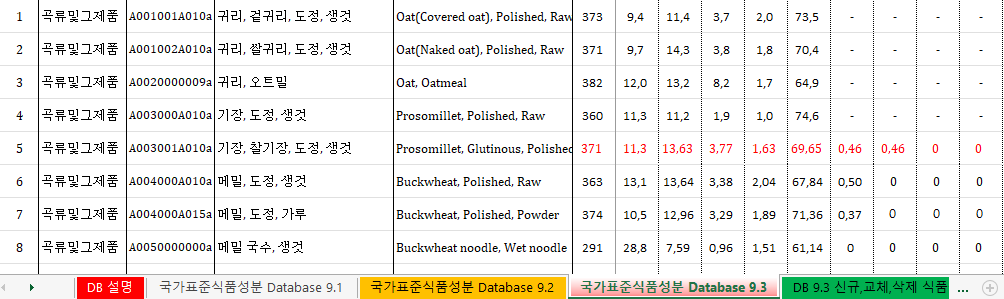
\includegraphics[width=\textwidth]{Figures/fsk-data.png}
  \caption{%
    Excel file provided by Food Safety Korea
  }
  \label{fig:fsk-data}
\end{figure}

\section{Development}

In this section, we will discuss mainly about the two different IDEs used during the programming and development of the mobile application: Visual Studio Code and Android Studio.

\subsection{Visual Studio Code}

Visual Studio Code \cite{noauthor_documentation_2021}, abbreviated as VS Code, is a code editor developed by Microsoft. It is free, open-source, and since its release in 2015 it has quickly risen to become the most popular source code editor by a great margin \cite{noauthor_stack_nodate}. It is highly customisable, with a library of plugins that provides support for virtually any programming language available. Figure \ref{fig:vscode-logo} depicts Visual Studio Code's logotype.

\begin{figure}[h]
  \centering
  
\includegraphics[width=0.25\textwidth]{Figures/vscode-logo.png}
  \caption{%
    Visual Studio Code's logotype
  }
  \label{fig:vscode-logo}
\end{figure}

Visual Studio Code is one of the two IDEs (along with Android Studio) that is officially supported for Flutter development, with a plugin that adds most of the functionality built in Android Studio such as hot-reload, support for Dart and several other coding and debugging options. Because of its simplicity, high modularity, widespread usage and complete support for Flutter, it was chosen as the text editor of preference during most of the development. We can see an screenshot of Visual Studio Code's interface in Figure \ref{fig:vscode-screen}.

\begin{figure}[h]
  \centering
  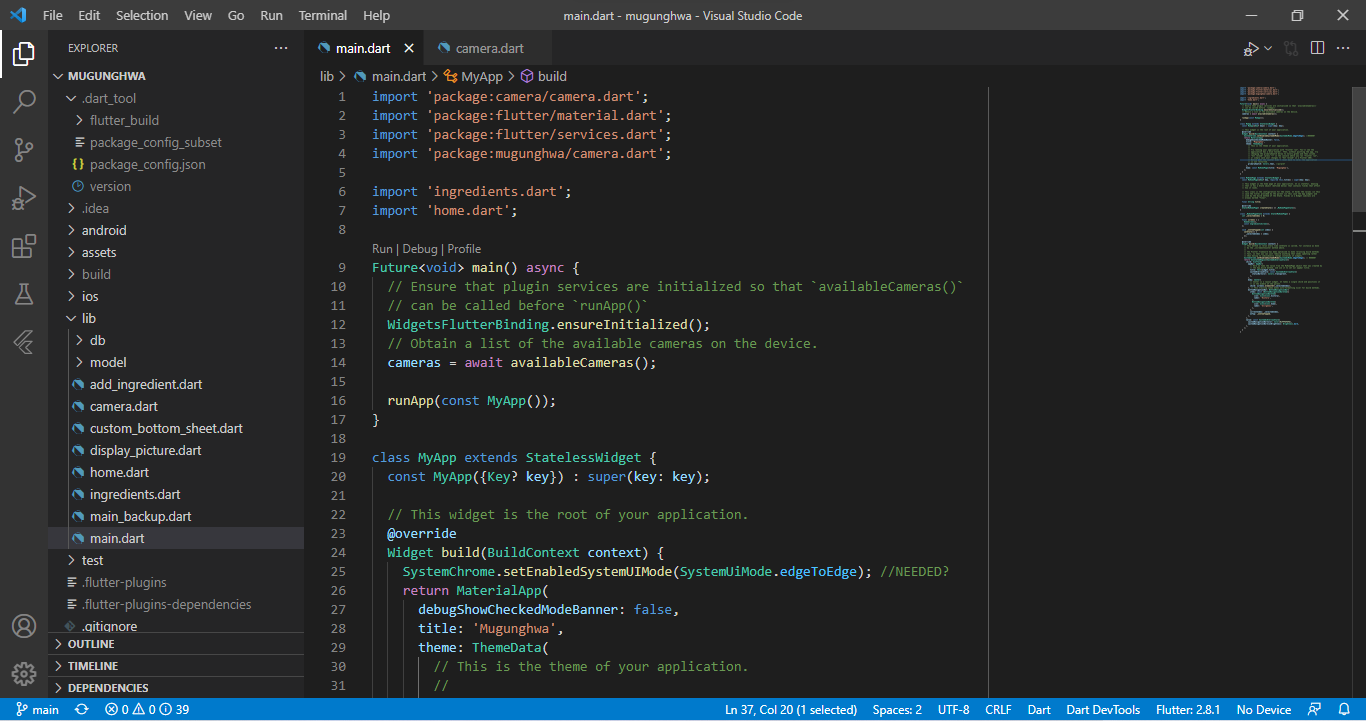
\includegraphics[width=\textwidth]{Figures/vscode-screen.png}
  \caption{%
    Visual Studio Code's user interface
  }
  \label{fig:vscode-screen}
\end{figure}

It is worth noting that Visual Studio Code also implements out-of-the-box support for version control systems such as Git. This way, we can commit, pull or push changes to our repository directly from VS Code interface without having to deal with a separate CLI interface.

\subsection{Android Studio}

Android Studio \cite{noauthor_introduccion_2021} is the official IDE for the Android platform, and therefore is also developed and maintained by Google. It was released in 2014 and replaced Eclipse as the standard IDE for Android app development. Though it natively only supports Java, Kotlin and C++, Dart support as well as most of the needed Flutter functionality can be added through the Flutter official plugin. Its logotype is shown in Figure \ref{fig:android-studio}.

\begin{figure}[h]
  \centering
  
\includegraphics[width=0.5\textwidth]{Figures/android-studio.png}
  \caption{%
    Android Studio's logotype
  }
  \label{fig:android-studio}
\end{figure}

Despite it being the default IDE for Android, Android Studio was only used during the initial stages of this project. This is due to it being way more heavy on resources than Visual Studio Code, making it more time inefficient for its usage on a machine with limited resources like the one used during development. Figure \ref{fig:android-studio-screen} shows the user interface of Android Studio.

\begin{figure}[h]
  \centering
  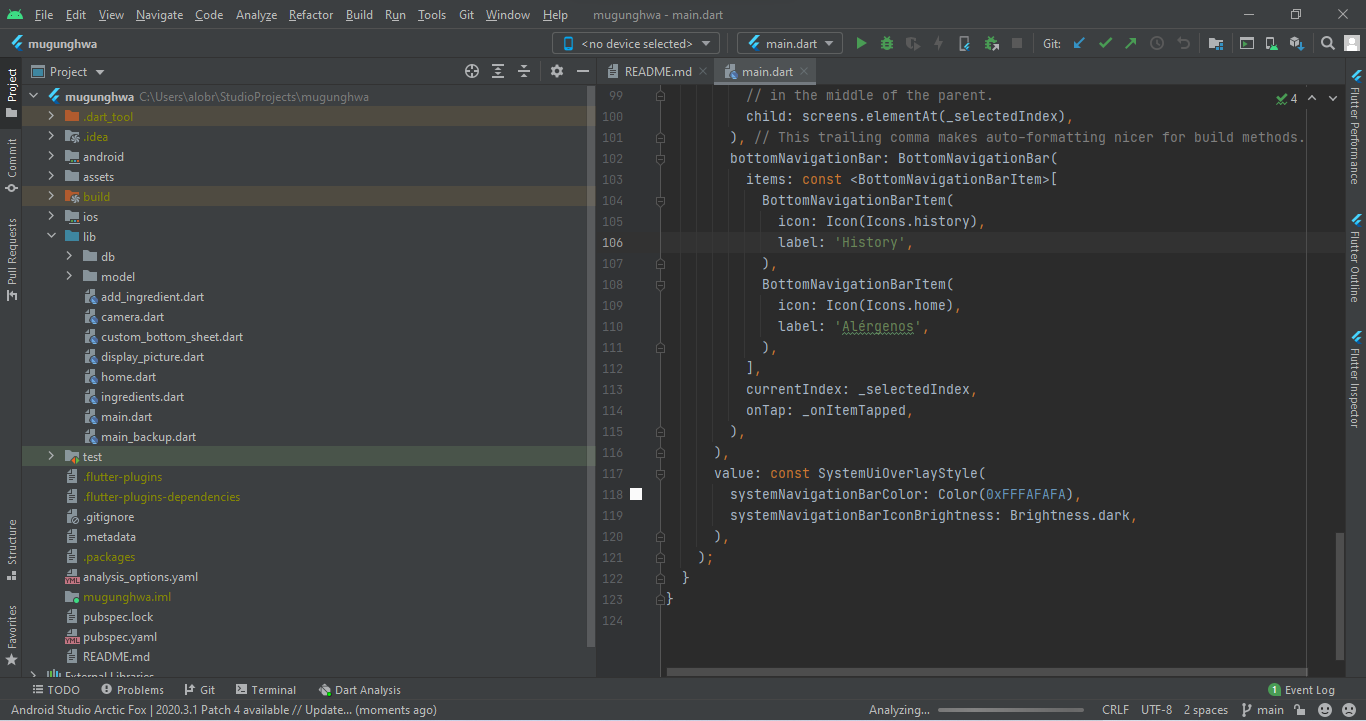
\includegraphics[width=\textwidth]{Figures/android-studio-screen.png}
  \caption{%
    Android Studio's user interface
  }
  \label{fig:android-studio-screen}
\end{figure}

It was still used occasionally because it offers way more Android-specific functions than our Visual Studio Code configuration. For example, it was used to create Android virtual devices (AVDs) for testing purposes.

\section{Version control}

In this section we will briefly describe the tools used to maintain a version control of the project source files and documentation.

\subsection{Git}

For efficiently keeping track of any changes made in the project code and documentation files we utilized Git \cite{noauthor_git_2021}. Git is a free and open-source version control software whose main purpose is registering any changes made on the project files, allowing to coordinate and synchronize the work across members of a team that are working on the same code. Git's logotype is shown in Figure \ref{fig:git}.

\begin{figure}[h]
  \centering
  
\includegraphics[width=0.5\textwidth]{Figures/git-logo.png}
  \caption{%
    Git's logotype
  }
  \label{fig:git}
\end{figure}

Even though the team is solely composed of one member, Git has been used to rollback to previous versions whenever needed, as well as to easily share any modifications with the project's director. It was also chosen because of the multiple integrations available with other tools in the stack such as Visual Studio Code or Overleaf. 

Git is also a distributed system, which means that the complete codebase (the files generated by the version control) is stored on the user computer instead of only on the server like in centralized client-server systems like such as Subversion \cite{noauthor_apache_nodate} or CVS \cite{noauthor_cvs_nodate}. Figure \ref{fig:git-repo} shows the repository structure and the files generated by Git in Git Bash, a CLI tool provided by the default installation.

\begin{figure}[h]
  \centering
  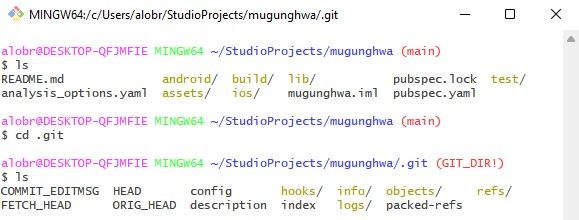
\includegraphics[width=0.75\textwidth]{Figures/git-repo.png}
  \caption{%
    Repository and files generated by Git
  }
  \label{fig:git-repo}
\end{figure}

Despite being a decentralized system, we also made use of a centralized platform for hosting our Git repository while having access to several additional features such as issue tracking, Kanban boards, \textit{wikis}, etc. This centralized hosting service is GitHub.

\subsection{GitHub}

GitHub \cite{noauthor_githubcom_2021} is a platform dedicated to provide hosting and version control services using Git for the source code of any software project. It was founded in 2008 and in 2018 it was acquired by Microsoft, which was already hosting over 4.500 of its projects on the platform. The projects stored in GitHub servers are typically public and available for everyone, as it is mainly a platform dedicated for open-source and collaborative projects. However, it also offers the possibility to open private repositories, first as a paid feature but available for free users too since April 2020. Figure \ref{fig:github-logo} shows GitHub's logotype.

\begin{figure}[h]
  \centering
  
\includegraphics[width=0.5\textwidth]{Figures/github-logo.png}
  \caption{%
    GitHub's logotype
  }
  \label{fig:github-logo}
\end{figure}

GitHub offers a wide array of functionalities that extend the basic Git usage, including \textit{wikis}, web pages, graphs and chart views for repository statistics, social features such as followers or stars, Kanban boards and even a cloud IDE based on Visual Studio Code. Out of these functionalities, Kanban boards and issue tracking were used extensively as explained in Chapter \ref{chapter4}. Besides, the platform was used to communicate issues in other pertinent repositories such as the Flutter one\footnote{Available at: \url{github.com/flutter/flutter}}, which is the 15th top repository by number of stars \cite{noauthor_repositories_nodate}. A screenshot of the GitHub repository used for hosting the code of the mobile application can be seen on Figure \ref{fig:github-repo}.

\begin{figure}[h]
  \centering
  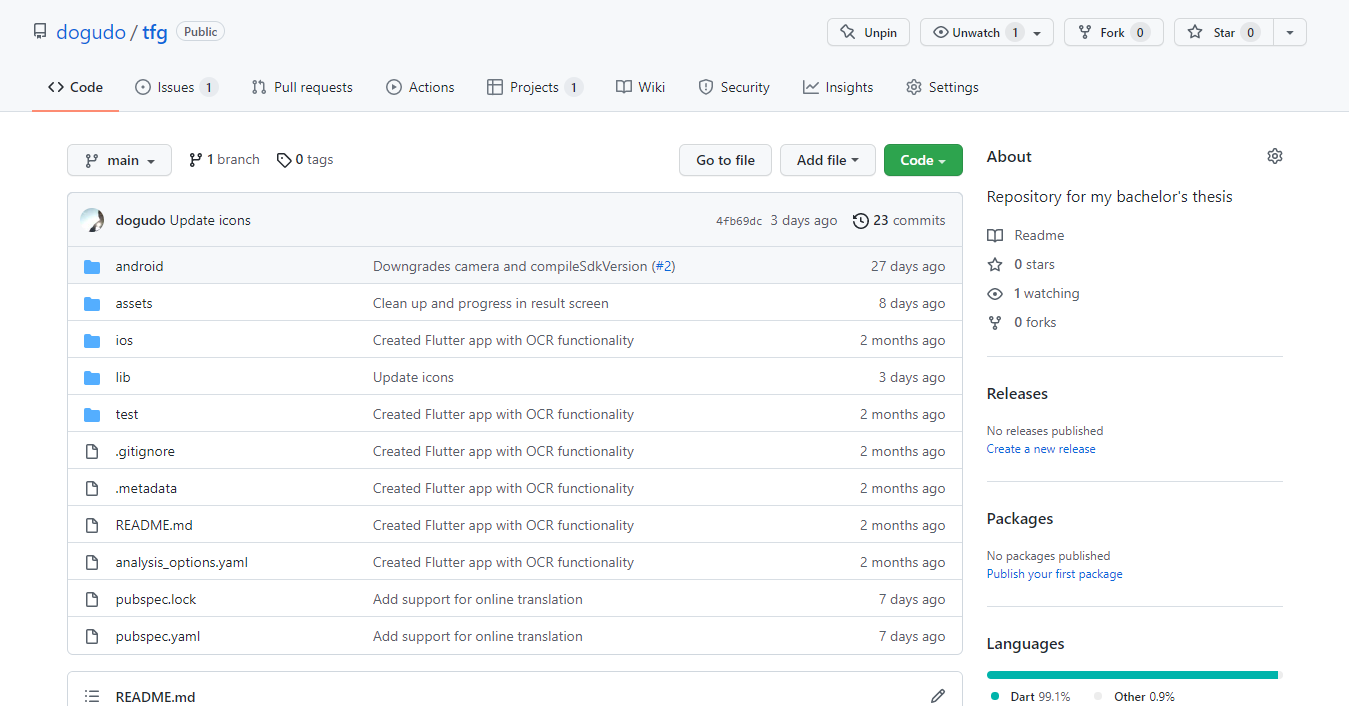
\includegraphics[width=\textwidth]{Figures/github-repo.png}
  \caption{%
    This project's repository hosted in GitHub
  }
  \label{fig:github-repo}
\end{figure}

For this project, two separate GitHub repositories were used. These are publicly available at the following locations:

\begin{itemize}
\item \texttt{tfg}, including the source files, database and other assets for the mobile application, is available at \url{github.com/dogudo/tfg}.
\item \texttt{tfg-report}, including the \LaTeX code of this report, is available at \url{github.com/dogudo/tfg-report}.
\end{itemize}

\section{Documentation}

In this section we will describe the tools that were used to compile, compose and write the documentation provided for the project, such as this report along with the charts and diagrams.

\subsection{\LaTeX}

\LaTeX\ \cite{noauthor_latex_nodate} is a high-quality typesetting ant text composing language, particularly oriented to the production of academic documents. As such, it has been widely adopted by the scientific community since its initial release back in 1984 and constitutes a de facto standard. It's logotype can be seen in Figure \ref{fig:latex}.

\begin{figure}[h]
  \centering
  
\includegraphics[width=0.5\textwidth]{Figures/latex.png}
  \caption{
    Latex's logotype.
  }
  \label{fig:latex}
\end{figure}

\LaTeX\ supports a great amount of plugins and commands to extend the base language and facilitate some functionalities such as including images, captions, text in non-Latin like \textit{hangeul}, import PDF pages from other documents, rotate figures, etc. In Listing \ref{lst:latex} we can see an example of the \LaTeX\ code needed to output both the previous figure and this paragraph.

\begin{code}
\begin{minted}[
breaklines,
frame=lines,
framesep=2mm,
baselinestretch=1.2,
fontsize=\footnotesize,
linenos
]{tex}
\begin{figure}[h]
  \centering
  \includegraphics[width=0.5\textwidth]{Figures/latex.png}
  \caption{
    Latex's logotype.
  }
  \label{fig:latex}
\end{figure}

\LaTeX\ supports a great amount of plugins and commands to extend the base language and facilitate some functionalities such as including images, captions, text in non-Latin like \textit{hangeul}, import PDF pages from other documents, rotate figures, etc. In this project, it was the typesetting language of choice to compose this document. Figure \ref{lst:latex} shows an example of the \LaTeX\ code needed to output this paragraph.
\end{minted}
\caption{Example of \LaTeX\ code}
\label{lst:latex}
\end{code}

\vskip\baselineskip
One of the main advantages of \LaTeX\ is that it has a large community and there are many templates readily available, which allows the user to focus on the writing task without having to worry about the structure and format of the document.

For this report we used a modified version of the \texttt{latex-mimosis} template by Bastian Rieck \cite{rieck_latex-mimosis_2022}, which is designed for typesetting thesis-like documents and is publicly hosted on a GitHub repository\footnote{Available at: \url{github.com/Pseudomanifold/latex-mimosis}}.

\subsection{Overleaf}

Overleaf \cite{noauthor_documentation_nodate} is a \LaTeX\ editor available on the cloud. This is particularly interesting because it allows the use of \LaTeX\ without needing to perform a full installation on the user device, which can usually be very heavyweight. Another interesting feature of this editor is that it allows collaborative editing, in a similar way as other options like Google Docs. Overleaf's logotype is seen in Figure \ref{fig:overleaf}.

\begin{figure}[h]
  \centering
  \includegraphics[width=0.4\textwidth]{Figures/overleaf.png}
  \caption{
    Overleaf's logotype.
  }
  \label{fig:overleaf}
\end{figure}

It was chosen as the editor of choice for writing this report in order to save time, as the package management when using other client-based options like TeXmaker or Lyx can often get quite tedious. Another needed feature about Overleaf is its direct integration with GitHub, allowing to commit and push changes from the browser. This also allows us to keep a backup of the document in the cloud in order to prevent any possible loss of data. A screenshot of Overleaf's editor view is shown in Figure \ref{fig:overleaf-screen}.

\begin{figure}[h]
  \centering
  \includegraphics[width=\textwidth]{Figures/overleaf-screen.png}
  \caption{
    Overleaf's user interface.
  }
  \label{fig:overleaf-screen}
\end{figure}

\subsection{Zotero}

Zotero \cite{noauthor_zotero_nodate} is the open-source bibliography manager that has been used to collect the papers and documentation referenced through this document. It is multi-platform and allows for synchronizing the library across devices by uploading to a cloud with up to 300 MB for free. Zotero's logotype is shown in Figure \ref{fig:zotero}.

\begin{figure}[h]
  \centering
  \includegraphics[width=0.4\textwidth]{Figures/zotero.png}
  \caption{
    Zotero's logotype.
  }
  \label{fig:zotero}
\end{figure}

Zotero was chosen over other alternatives because it simplifies the workflow for adding new references into the document. The cloud is one of its main strengths, as it can be used to seamless integrate the library into Overleaf and seamlessly update it whenever any addition is made. It also generates automatically the correct format for the bibliography style specified, IEEE in this case.

\subsection{Diagrams.net}

Diagrams.net \cite{noauthor_diagram_nodate}, most commonly known for its former name draw.io, is a free and open-source tool for drawing any kind of diagrams online. Its logotype can be seen in Figure \ref{fig:drawio}.

\begin{figure}[h]
  \centering
  \includegraphics[width=0.25\textwidth]{Figures/drawio.png}
  \caption{
    Diagrams.net logotype.
  }
  \label{fig:drawio}
\end{figure}

It was used to produce most of the diagrams, figures and schemas included in this document. The main reason for using diagrams.net is its versatility and ease of use. Like in the case of Overleaf, we can use diagrams.net from any device with access to a browser and save our designs in the cloud, allowing us to continue the work from any other platform. Though it is not the most professional tool available, it is more than sufficient for the types of diagrams needed and is particularly well suited for software development-related diagrams.

\subsection{Microsoft Project}

Lastly, Microsoft Project \cite{noauthor_project_nodate} is a project administration software dedicated to assist in most of the management processes like the planning of tasks or the handling of resources. Although it is usually available under a paid subscription, it is freely available for university students under the Azure for Education programme. Figure \ref{fig:msproject} shows Microsoft Project's logo.

\begin{figure}[h]
  \centering
  \includegraphics[width=0.25\textwidth]{Figures/msproject.png}
  \caption{
    Microsoft Project's logotype.
  }
  \label{fig:msproject}
\end{figure}

Microsoft Project was solely used during this project to produce the Gantt diagrams in Chapter \ref{chapter3} as well as to determine the time distribution of the several tasks that were defined. 
    \chapter{Project development}
\label{chapter6}

In this chapter we will discuss and deepen in all of the tasks and subprocesses that took part in the completion of this project. We will also thoroughly detail all of the steps that were followed in order to complete these steps and materialize the mobile application.
    \chapter{Results}
\label{chapter7}

In this chapter we will exhibit some screenshots of the main screens of NokScanner, detailing the most relevant elements of the user interface and introducing the final design of the mobile application. We will also present some practical use cases in order to test the accuracy of the app.

\section{Device specifications}

This section details the main characteristics of the testing device used to verify the adequate working of the mobile application, to be taken as reference in case of any possible issues that may arise when using the app on other devices.

During the development of this project, the only device available for testing was the author personal Android device. Therefore, this app has not been tested on an iOS device (iPhone, iPad, etc.) and may not work on one without further troubleshooting, which could be explored and developed as future work. The specifications of the device used are the following:

\begin{itemize}
\item \textbf{Device model}: Samsung A51 5G
\item \textbf{Operative system}: Android 11
\item \textbf{Processsor}: Samsung Exynos 980 (Octa-core, 2x 2.2GHz + 6x 1.8GHz, 64-bit)
\item \textbf{Internal memory}: 6 GB RAM
\item \textbf{Storage memory}: 128 GB
\item \textbf{Screen}: 6.5 inches, 2400 x 1080 pixels
\item \textbf{Camera}: 48MP quad camera (back), 32MP camera (front)
\end{itemize}

\section{User interface}

Below are presented several screenshots of the mobile app showcasing the different screens and components of the user interface.

\subsection{History}

This is the screen loaded when starting the app. An empty history shows a prompt to try to scan for the first time (Figure \ref{fig:history-empty}). After some scans, the history shows the recent entries sorted by date, also displaying their name and image (Figure \ref{fig:history}).

\begin{figure}[h]
    \begin{subfigure}{0.5\textwidth}
        \centering
        \includegraphics[width=0.9\linewidth]{Figures/Screenshot/history_empty.jpg} 
        \caption{Empty history}
        \label{fig:history-empty}
    \end{subfigure}
    \begin{subfigure}{0.5\textwidth}
        \centering
        \includegraphics[width=0.9\linewidth]{Figures/Screenshot/history.jpg}
        \caption{Populated history}
        \label{fig:history}
    \end{subfigure}
    \caption{History screen}
    \label{fig:history2}
\end{figure}

By tapping the heart icon, the user can also save some of this entries and keep them inside a dedicated "favorites" view (Figure \ref{fig:favs}). This view is accessed by clicking the heart outline icon on the app bar.

\begin{figure}[h]
  \centering
  \includegraphics[width=0.5\textwidth]{Figures/Screenshot/favs.jpg}
  \caption{%
    Favorites screen
  }
  \label{fig:favs}
\end{figure}

\clearpage

\subsection{Help and FAQ}

The help screen can be accessed through almost all of the screens in the app through a question mark button at the top right. This screen has 3 panels (Figure \ref{fig:help-collapse}) that can be expanded to show some information about the correct usage of the app and some precautions and safety disclaimers for the user (Figure \ref{fig:help}).

\begin{figure}[h]
    \begin{subfigure}{0.5\textwidth}
        \centering
        \includegraphics[width=0.9\linewidth]{Figures/Screenshot/help_collapse.jpg} 
        \caption{Collapsed panels}
        \label{fig:help-collapse}
    \end{subfigure}
    \begin{subfigure}{0.5\textwidth}
        \centering
        \includegraphics[width=0.9\linewidth]{Figures/Screenshot/help.jpg}
        \caption{Expanded panels}
        \label{fig:help}
    \end{subfigure}
    \caption{Help screen}
    \label{fig:help2}
\end{figure}

\clearpage

\subsection{Camera and gallery}

By tapping the scanner button on the main screen, the user is taken to the camera or scanner view (Figure \ref{fig:camera}). This screen is composed of a full-screen camera preview, a button to take the picture, and action buttons on the top bar to toggle the flash, go to the help view or select a previous photo from the image picker (Figure \ref{fig:image-picker}). This image picker is an Android native element, and upon choosing a picture the user is taken to the results view.

\begin{figure}[h]
    \begin{subfigure}{0.5\textwidth}
        \centering
        \includegraphics[width=0.9\linewidth]{Figures/Screenshot/camera.jpg} 
        \caption{Camera}
        \label{fig:camera}
    \end{subfigure}
    \begin{subfigure}{0.5\textwidth}
        \centering
        \includegraphics[width=0.9\linewidth]{Figures/Screenshot/image_picker.jpg}
        \caption{Image picker}
        \label{fig:image-picker}
    \end{subfigure}
    \caption{Camera and image picker screens}
    \label{fig:camera2}
\end{figure}

\clearpage

\subsection{Scanning results}

The scanning results screen is composed of a small thumbnail of the image taken, which can be tapped to expand it to full screen, an editable field to input the title that will show on the history, the date and time, and a distinct banner showing the number of unwanted ingredients found. Below this elements, there is either a list of all the unwanted ingredients found in the packaging along with their Korean names (Figure \ref{fig:scan-warn}), or a "no matches found" text along with a disclaimer to double-check manually (Figure \ref{fig:scan-pass}).

\begin{figure}[h]
    \begin{subfigure}{0.5\textwidth}
        \centering
        \includegraphics[width=0.9\linewidth]{Figures/Screenshot/scan_pass.jpg} 
        \caption{No unwanted ingredients}
        \label{fig:scan-pass}
    \end{subfigure}
    \begin{subfigure}{0.5\textwidth}
        \centering
        \includegraphics[width=0.9\linewidth]{Figures/Screenshot/scan_warn.jpg}
        \caption{4 unwanted ingredients}
        \label{fig:scan-warn}
    \end{subfigure}
    \caption{Scanning results screen}
    \label{fig:scan}
\end{figure}

\clearpage

\subsection{Text translation}

If the user taps the bottom right icon of the scan results screen, a modal sheet will pop up displaying both the recognized text in Korean as well as the translated text in English (Figure \ref{fig:translate}). This way the user can manually double-check if they suspect a synonym for an unwanted ingredient may have been left unrecognized by the application.

\begin{figure}[h]
  \centering
  \includegraphics[width=0.5\textwidth]{Figures/Screenshot/papago.jpg}
  \caption{%
    Translation modal sheet
  }
  \label{fig:translate}
\end{figure}

\clearpage

\subsection{Allergens}

In the allergens view, the user can see all of the active filters or ingredients to be detected by the app when running a scan (Figure \ref{fig:ingredients}). Every entry is shown with both the names in English and Korean, and they can be disabled at any moment by clicking the trash can icon to the right. The user can add more of these filters at any time by tapping the add (+) button.

\begin{figure}[h]
  \centering
  \includegraphics[width=0.5\textwidth]{Figures/Screenshot/ingredients.jpg}
  \caption{%
    Allergens screen
  }
  \label{fig:ingredients}
\end{figure}

\clearpage

When tapping the add button on the bottom right, the user can add a new unwanted ingredient to filter when scanning a product. When typing the English name, suggestions from the pre-built ingredients database are shown (Figure \ref{fig:ingredients-autocomplete}). If any of these is selected, the Korean name is autocompleted too (Figure \ref{fig:ingredients-add}). If not, the Korean name field will be guessed using the translation API. In any case, the user can manually modify both fields and press the save button on the top right to add the ingredient.

\begin{figure}[h]
    \begin{subfigure}{0.5\textwidth}
        \centering
        \includegraphics[width=0.9\linewidth]{Figures/Screenshot/ingredients_autocomplete.jpg} 
        \caption{Ingredient suggestions}
        \label{fig:ingredients-autocomplete}
    \end{subfigure}
    \begin{subfigure}{0.5\textwidth}
        \centering
        \includegraphics[width=0.9\linewidth]{Figures/Screenshot/ingredients_add.jpg}
        \caption{Autocompleted fields}
        \label{fig:ingredients-add}
    \end{subfigure}
    \caption{Add ingredient screen}
    \label{fig:ingredients2}
\end{figure}

\clearpage
    \chapter{Conclusions and future work}
\label{chapter8}

\section{Conclusions}

\section{Future work}
    
    \appendix
    \chapter{Gantt diagrams}
\label{appendix:A}

\section{Planned Gantt diagram}

\begin{sidewaysfigure}
  \centering
  \includegraphics[width=\textwidth]{Figures/gantt_planned.pdf}
  \caption{%
    Gantt chart for the planned DFP schedule
  }
  \label{fig:gantt_planned}
\end{sidewaysfigure}

\clearpage

\section{Actual Gantt diagram}

\begin{sidewaysfigure}
  \centering
  \includegraphics[width=\textwidth]{Figures/gantt_actual.pdf}
  \caption{%
    Gantt chart for the actual DFP schedule
  }
  \label{fig:gantt_actual}
\end{sidewaysfigure}

% This ensures that the subsequent sections are being included as root
% items in the bookmark structure of your PDF reader.
\bookmarksetup{startatroot}
\backmatter

  \begingroup
    \let\clearpage\relax
    \glsaddall
    \printglossary[type=\acronymtype]
    \newpage
    \printglossary
  \endgroup

  \printindex
  \printbibliography
  
  \includepdf[]{Cover/ContraportadaTFG.pdf}
  
\end{document}